\chapterimage{slike/Primeri.jpg} 
% Chapter heading image
\chapter{Primeri laserjev}
\label{chap:Primeri}
V tem poglavju bomo spoznali nekaj najpomembnejših vrst laserjev.
V grobem laserje razlikujemo po aktivnem sredstvu 
(plin, trdna snov, organsko barvilo, polprevodnik), pri čemer tudi pri izbranem
sredstvu obstaja veliko različnih izvedb in načinov delovanja. Za vsak 
obravnavani primer bomo navedli osnovne karakteristike, v podrobnosti 
izvedbe pa se ne bomo spuščali. 

\section{Laserski sistemi}
\index{Laserski sistemi}
Laser \index{Laser} je lahko dokaj preprosta naprava, z malo sestavnimi deli, 
lahko pa je zelo velik in zapleten sistem. Večina laserskih sistemov
je sestavljena iz osnovnega laserja, ki ni posebno močan, a daje kvaliteten
snop svetlobe, in iz enega ali več ojačevalnikov. V njih se svetloba 
ojačuje v sredstvu, ki je enako kot v osnovnem laserju in ki je v kolikor 
mogoče visokem stanju obrnjene zasedenosti. V več ojačevalnih korakih 
se tako doseže zelo velika svetlobna moč. 

Pri velikih laserskih močeh nastopi vrsta novih težav. Da gostota 
svetlobnega toka ne povzroča poškodb optičnih komponent, mora 
premer ojačevanega snopa (in s tem premer vseh vmesnih ojačevalnih stopenj) 
naraščati. Na zadnjih stopnjah največjih laserskih sistemov je 
premer snopa lahko večji od pol metra, kar seveda pomeni, da morajo imeti tolikšno odprtino 
tudi vse ostale optične komponente. Poleg tega je
treba skrbno paziti, da se odbita svetloba ne vrača v prejšnji
ojačevalnik ali v osnovni laser in s tem moti njegovo delovanje. Med
posamezne ojačevalne stopnje zato damo optične izolatorje, ki temeljijo na Faradayevem
pojavu vrtenja polarizacije v snovi z magnetnim poljem.

\begin{figure}[h!]
\centering
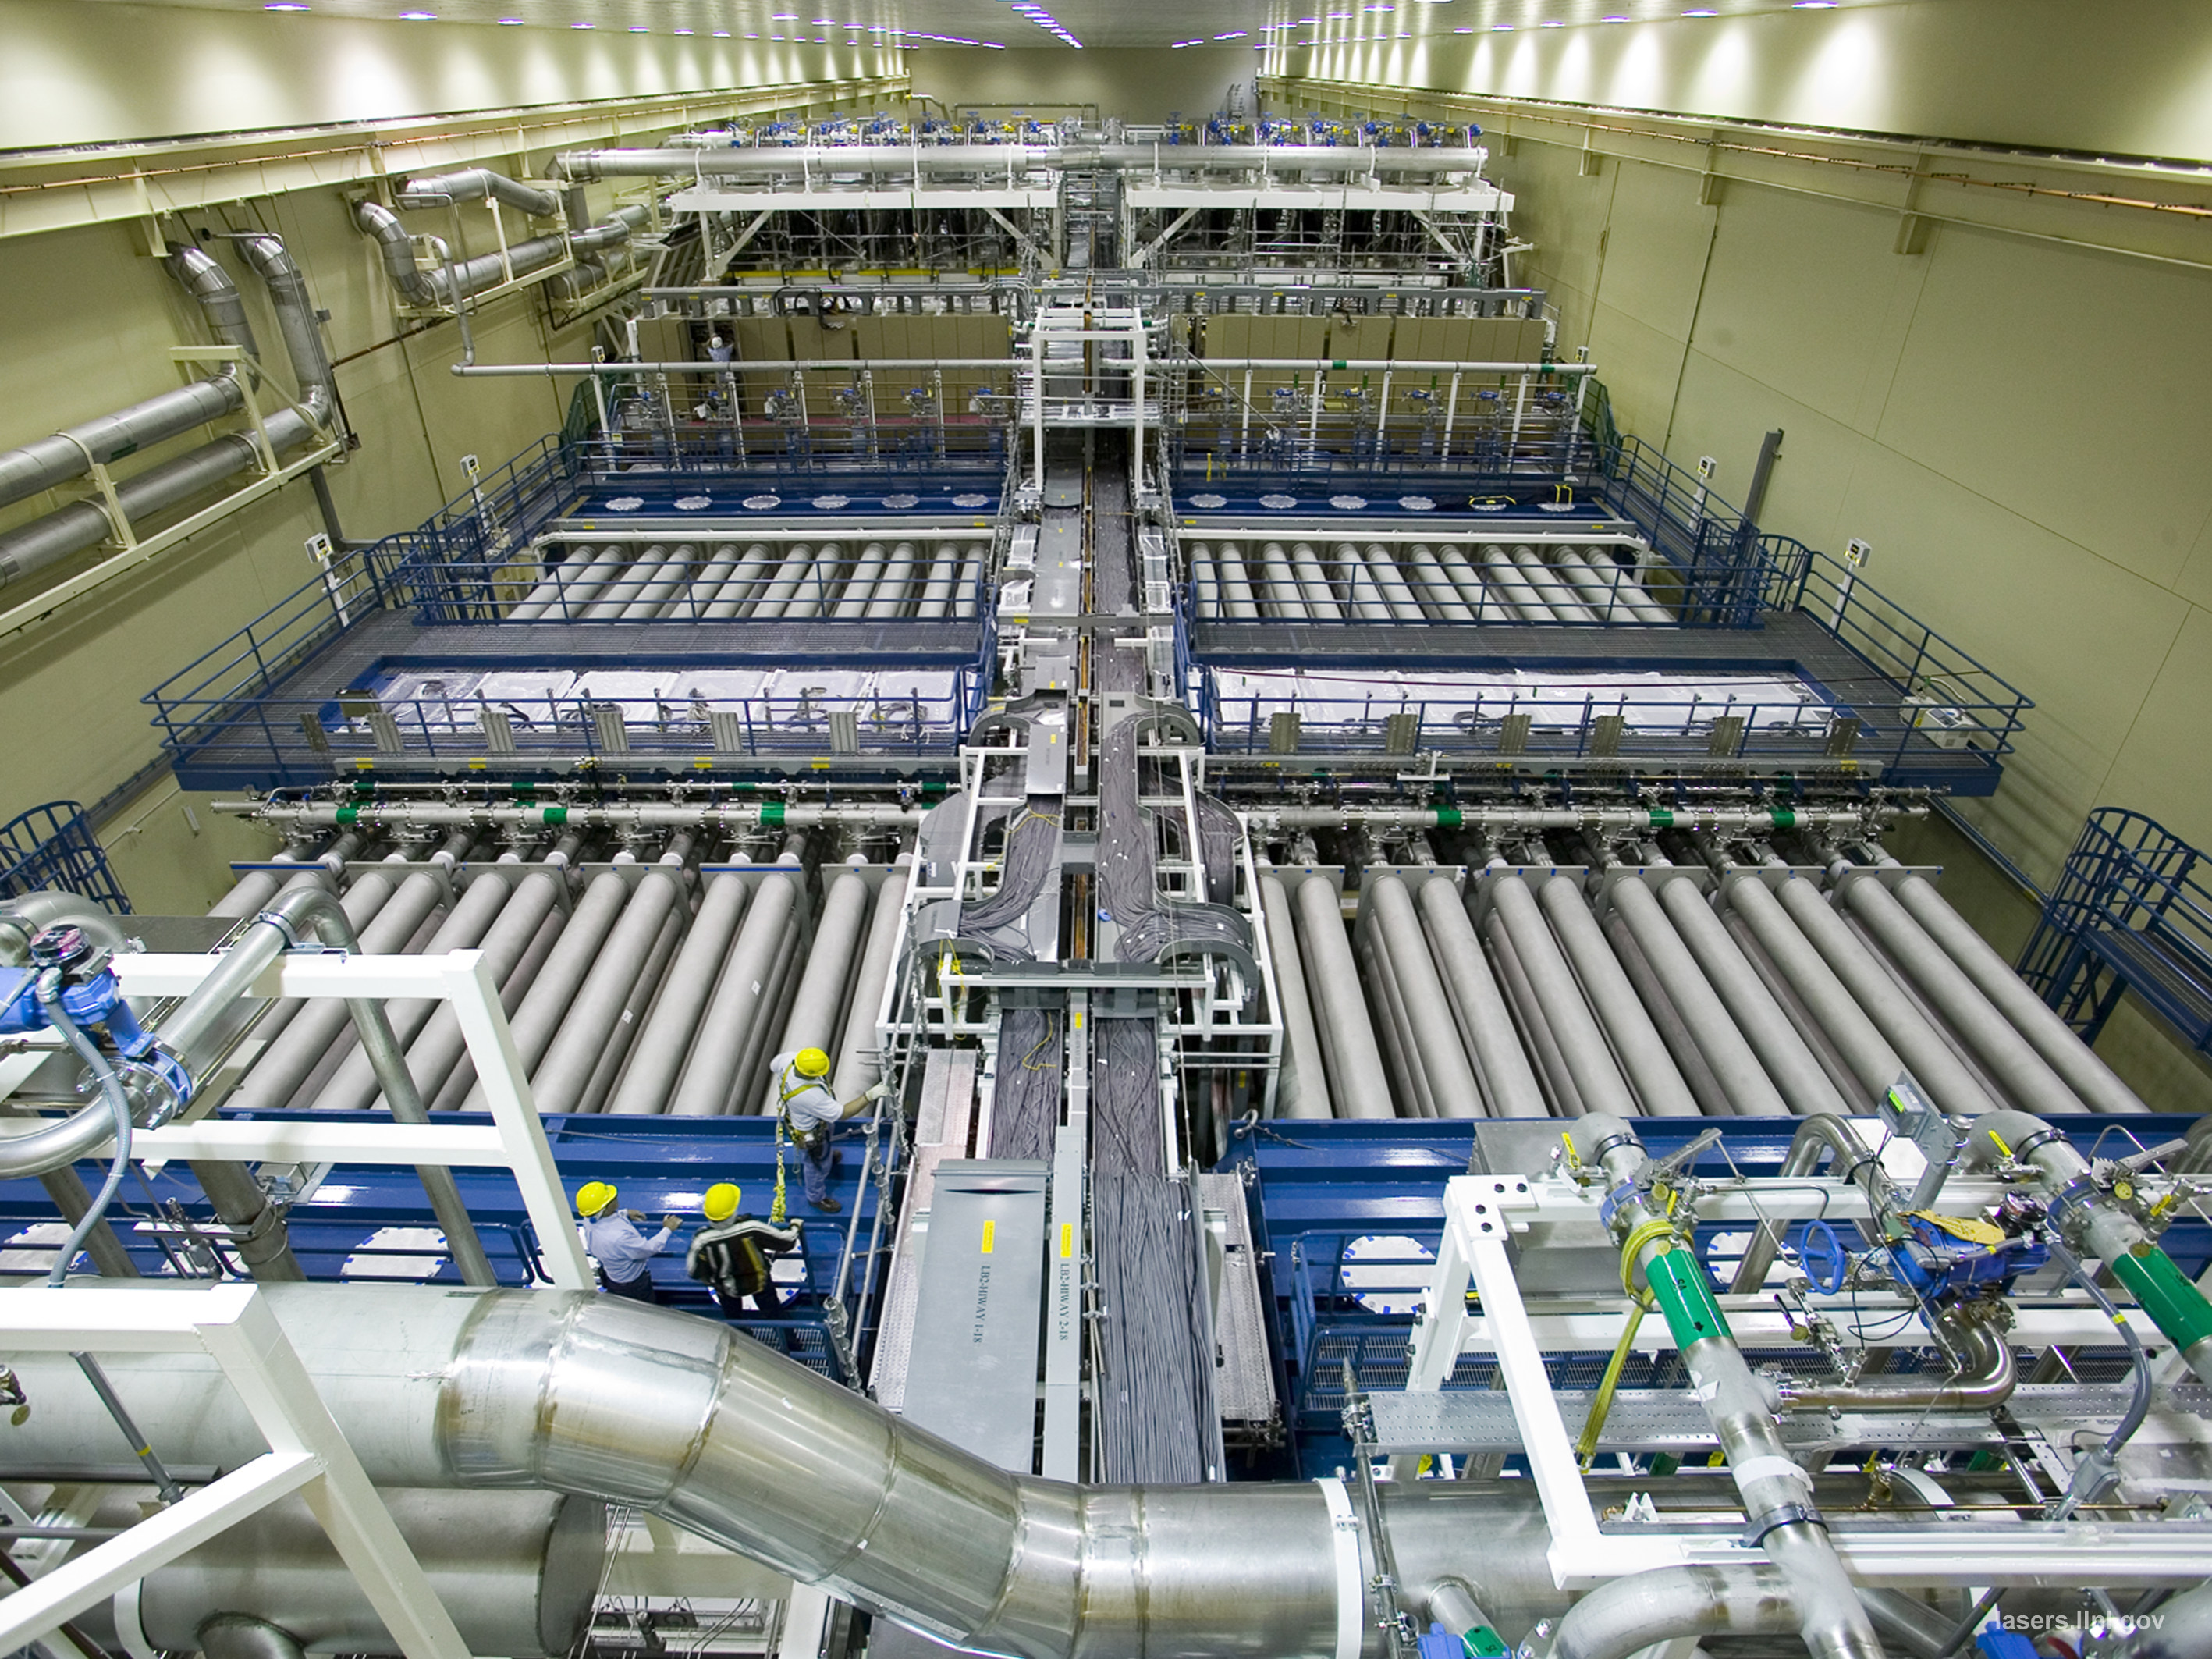
\includegraphics[width=100truemm]{slike/07_NIF_Laser_Bay.jpg}
\caption{Eden najmočnejših laserskih sistemov na svetu, ki doseže 
$500~\si{\tera\watt}$ moči v sunku. \\Vir: National Ignition Facility, Livermore, Kalifornija.}
\label{fig:NIF}
\end{figure}

Moči svetlobe, ki jih oddajajo najmočnejši laserski sistemi, imajo zelo velike
vrednosti. Najmočnejši zvezno delujoči laserji dosegajo moči prek 
$\sim 100~\si{\kilo\watt}$. Še bistveno večje moči dosegajo sunkovni laserji, 
saj lahko v sunku dosežejo moč tudi $\sim 10^{15}~\si{\watt}$. 
Vendar so sunki s tako veliko svetlobno močjo izredno kratki, tipično reda pikosekunde, tako da
znaša celotna energija v sunku ``le'' $\sim \si{\kilo\joule}$. Pomemben
parameter pri sunkovnih laserjih je tudi čas, ki poteče med dvema zaporednima
sunkoma (repeticija). Najmočnejši laserski sistemi lahko izsevajo največ nekaj sunkov dnevno. 

\section{He-Ne laser}
\index{Laser!He-Ne}
Najprej si oglejmo helij-neon (He-Ne) laser, ki je bil prvi zvezno 
delujoči laser in je še danes zelo razširjen. Najpogosteje deluje 
pri valovni dolžini $632,8~\si{\nano\metre}$ v rdečem delu spektra, lahko 
pa tudi pri infrardečih $1,15~\si{\micro\metre}$ in 
$3,39~\si{\micro\metre}$ ter nekaterih drugih\index{Infrardeče valovanje}
valovnih dolžinah v oranžnem in zelenem delu spektra. Laser deluje v zveznem 
načinu delovanja s tipičnimi močmi $0,5$--$100~\si{\milli\watt}$.

Ojačevalno sredstvo je plin, mešanica helija in neona, katerih relevantni
energijski nivoji so prikazani na sliki~(\ref{fig:HeNeE}). 
\index{Energijski nivoji!He-Ne}
\index{Trinivojski sistem}
Atome helija
s trki z elektroni vzbudimo v eno izmed dveh dolgoživih metastabilnih stanj $2^3S$ ali
$2^1S$ z razpadnima časoma $0,1~\si{\milli\second}$ in $5~\si{\micro\second}$.
Ti dve stanji slučajno praktično sovpadata z dvema stanjema neona ($4s$ in $5s$). 
Ko heliju dodamo neon, se energija s trki 
prenese z vzbujenih helijevih atomov na atome neona, ki s tem preidejo v 
že omenjeni vzbujeni stanji. Helijevi atomi se po trku vrnejo v osnovno stanje, od koder
jih lahko ponovno vzbudimo. Prenos energije z atomov helija na atome neona s trki je 
zelo učinkovit, zato zasedenost vzbujenih neonovih stanj hitro naraste. Ko preseže 
zasedenost nižjih vzbujenih stanj, pride do obrnjene zasedenosti. 

\begin{figure}[h]
\centering
\def\svgwidth{100truemm} 
\input{slike/07_HeNeE.pdf_tex}
\caption{Shema energijskih nivojev v He-Ne laserju. Nivoji helija so označeni
z modro in nivoji neona z zeleno, laserski prehodi pa z rdečimi barvami in pripisano
ustrezno valovno dolžino.}
\label{fig:HeNeE}
\end{figure}

Znano rdečo svetlobo He-Ne laserja z valovno dolžino $632,8~\si{\nano\metre}$ dobimo 
pri prehodu iz stanja $5s$ v eno od stanj $3p$. Pri tem je življenjski čas 
stanja $5s$ okoli $100~\si{\nano\second}$, stanja $3p$ pa okoli $10~\si{\nano\second}$, zato
se spodnji nivo s spontano emisijo hitro prazni  v metastabilno stanje $3s$. 
V njem se atomi nabirajo, saj so dipolni sevalni prehodi v osnovno stanje prepovedani,
in atomi le s trki ob steno cevi prehajajo v osnovno stanje. Da pospešimo
praznjenje nivoja $3s$ in omogočimo večjo obrnjeno zasedenost, moramo torej 
zmanjšati premer razelektritvene cevi. Zaradi gibanja atomov je spektralna 
črta Dopplerjevo razširjena\index{Dopplerjeva razširitev} ($\Delta \nu = 1,5~\si{GHz}$). 

Lasersko delovanje dobimo tudi pri prehodu iz $5s$ v stanje $4p$, pri katerem 
ima izsevana svetloba valovno dolžino $3,39~\si{\micro\metre}$. 
Ojačenje je za ta prehod celo precej večje kot za
prehod pri $632,8~\si{\nano\metre}$, deloma zaradi nižje frekvence 
(glej zvezo med Einsteinovima koeficientoma $A$ in $B$, enačba~\ref{4.27}), 
deloma pa zaradi kratke življenjske dobe spodnjega laserskega nivoja $4p$. 
Zato bi pričakovali, da bo He-Ne laser svetil v infrardečem delu in ne vidnem. 
To delno prepreči absorpcija v steklu, delno pa izgube namerno povečamo s selektivno odbojnostjo
resonatorskih zrcal, ki dvigne prag delovanja za $3,39~\si{\micro\metre}$ 
nad prag za $632,8~\si{\nano\metre}$. V laser lahko dodamo tudi
celico metana, ki infrardeč del svetlobe močno absorbira, vidnega pa ne.
Omenimo še prehode iz stanja $4s$, ki ga dosežejo neonovi atomi s trki
z vzbujenimi helijevimi atomi iz nivoja $2^3S$. Prehod $4s$ v $3p$, ki da svetlobo
pri $1,15~\si{\micro\metre}$, je bil prvi opaženi prehod v He-Ne laserjih.

Tipičen He-Ne laser je razmeroma preprosto zgrajen (sliki~\ref{fig:HeNeShema}
in \ref{fig:Iskra}).\index{Laser!zgradba}
V razelektritveni cevi (napetost  $\sim 1~\si{\kilo\volt}$), skozi
katero teče električni tok ($\sim 10~\si{\milli\ampere}$), 
se nahaja mešanica helija in neona v razmerju 
$5:1$--$10:1$. Skupni tlak v cevi je nizek, le okoli $3~\si{\milli\bar}$, 
cev pa je tipično dolga okoli $0,5~\si{\metre}$ s premerom $1$--$2~\si{\milli\metre}$.  
Cev na obeh straneh zapirata okni, ki sta nagnjeni za Brewstrov kot, 
tako da so izgube pri odboju za eno polarizacijo kar se da majhne.
Izhodna svetloba iz laserja je zato seveda polarizirana. V manjših laserjih
so namesto Brewstrovih oken na razelektritveno cev privarjena kar
resonatorska zrcala, zaradi česar so taki laserji nepolarizirani. 
Navadno je razelektritvena cev obdana z dvema ukrivljenima zrcaloma, 
ki imata zelo veliko odbojnost za izbrano valovno dolžino.
Nekaj tipičnih podatkov za He-Ne laser je zbranih v tabeli~(\ref{tab:Ar}).
\begin{figure}[h]
\centering
\def\svgwidth{100truemm} 
\input{slike/07_HeNeShema.pdf_tex}
\caption{Shema He-Ne laserja: R -- razelektritvena cev, IZ -- izhodno zrcalo, Z -- zrcalo
z veliko odbojnostjo, B -- Brewstrovi okni}
\label{fig:HeNeShema}
\end{figure}

\begin{figure}[h]
\centering
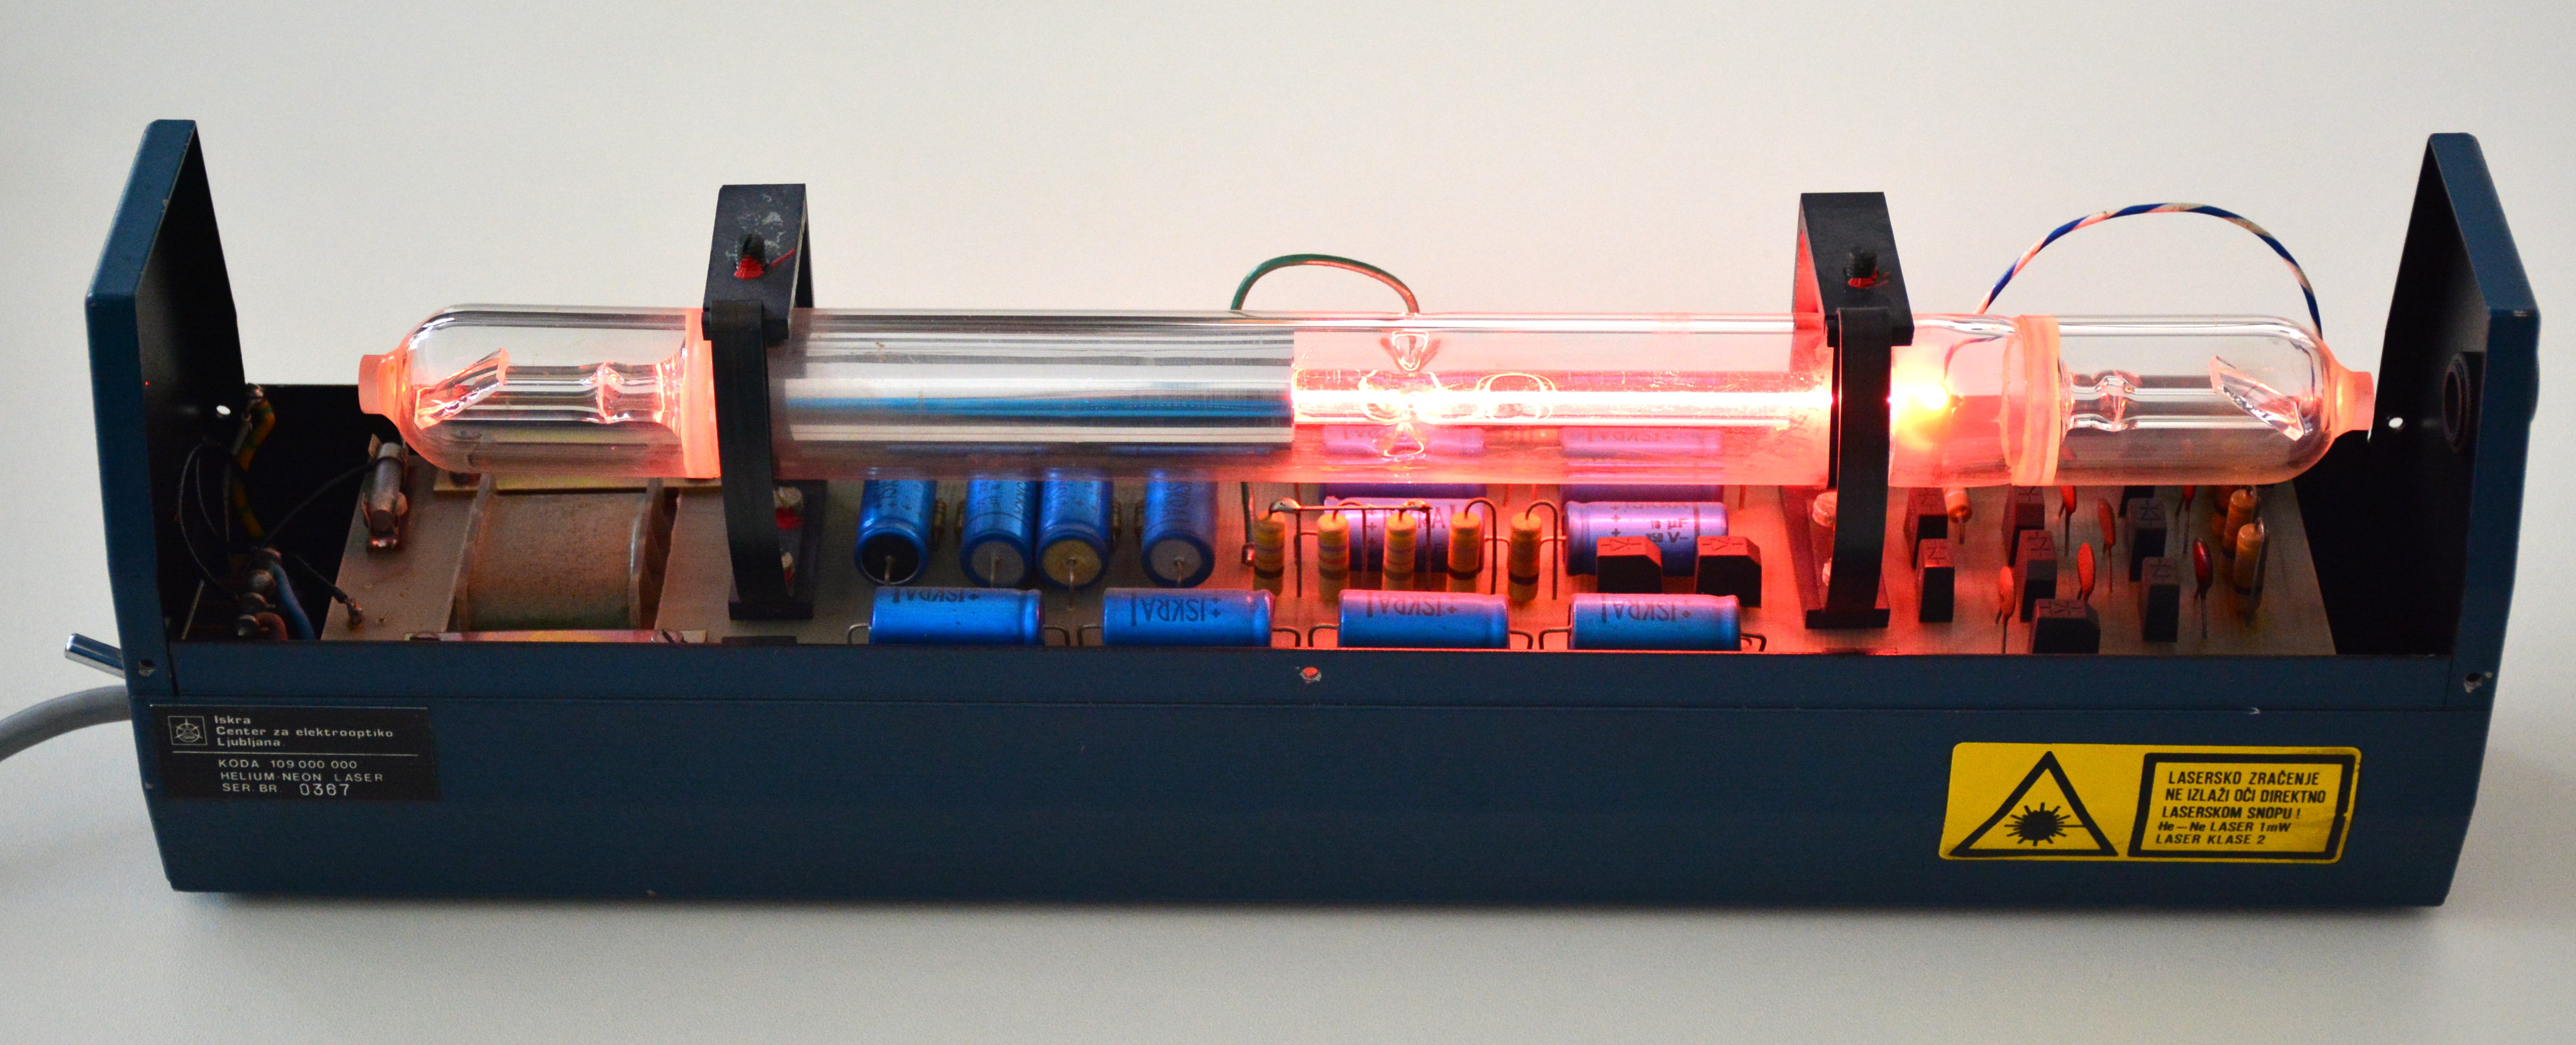
\includegraphics[width=120truemm]{slike/07_HeNe.jpg}
\caption{Primer starejšega He-Ne laserja, izdelanega v Sloveniji}
\label{fig:Iskra}
\end{figure}

He-Ne laserji so preprosti, stabilni, zanesljivi, poceni, imajo visoko kvaliteto žarka
in dolgo služijo (do 50 000 ur).
Danes jih sicer izrivajo polprevodniški laserji, vendar so še vedno v uporabi
v merilnih napravah, v optičnih čitalnih sistemih, v šolah, v raziskovalnih 
laboratorijih za interferometrijo, holografijo itd. Na njem je osnovan tudi 
standard za meter.

\section{Argonov ionski laser}
\index{Laser!argonov}
\index{Štirinivojski sistem}
Kot drugi primer plinskega laserja obravnavajmo argonov ionski (Ar$^+$) laser,
ki je najbolj poznan po zveznem delovanju v modrem in zelenem delu spektra pri 
valovnih dolžinah $488,0~\si{\nano\metre}$ in $514,5~\si{\nano\metre}$, deluje 
pa tudi v bližnjem ultravijoličnem delu spektra. Tipične moči delovanja argonovega laserja
so $100~\si{\milli\watt}$--$50~\si{\watt}$.\index{Ultravijolično valovanje}

Kot večino plinskih laserjev tudi tega črpamo z električnim tokom.
Atome argona vzbudimo s trki z elektroni v ione argona, ti pa z nadaljnjimi
trki preidejo v vzbujena stanja. Obrnjeno zasedenost
dosežemo med nivojema $4p$ in $4s$ (slika~\ref{fig:ArE}). 
Ta dva nivoja vsebujeta veliko podnivojev, zato je tudi prehodov med
njima zelo veliko. Argonov laser tako seva pri več kot tridesetih različnih
valovnih dolžinah, najznačilnejši sta že omenjeni 488~nm in 514,5~nm. 
Življenjski čas zgornjega nivoja je okoli $10~\si{ns}$, kar je približno 
desetkrat več od življenjskega časa spodnjega nivoja, od koder se ioni
z rekombinacijo z elektroni vrnejo v osnovno stanje atoma. Tudi pri tem laserju
je poglavitni vzrok za razširitev črte \index{Dopplerjeva razširitev}Dopplerjev 
pojav ($\Delta \nu = 3,5~\si{GHz}$).\index{Energijski nivoji!argon}

\begin{figure}[h]
\centering
\def\svgwidth{80truemm} 
\input{slike/07_ArE.pdf_tex}
\caption{Shema energijskih nivojev v Ar$^+$ laserju}
\label{fig:ArE}
\end{figure}

Argonov laser je v osnovi zgrajen podobno kot He-Ne laser. \index{Laser!zgradba}
V razelektritveni cevi
(tipična dolžina $1~\si{\metre}$ in premer $1$--$2~\si{\milli\metre}$)
se nahaja argon pri pritisku okoli $10~\si{\milli\bar}$. Ker gre pri 
vzbujanju atomov argona za dvostopenjski proces, mora biti električni tok, 
s katerim dosežemo obrnjeno zasedenost, precej velik, lahko tudi nekaj deset amperov. 
Pri tipični napetosti nekaj kV to pomeni, da so potrebne velike električne moči, 
pogosto več deset $\si{\kilo\watt}$, in močnejši argonovi laserji so zato zaradi 
velike količine odvečne toplote najpogosteje vodno hlajeni.

\begin{figure}[h]
\centering
\def\svgwidth{110truemm} 
\input{slike/07_ArShema.pdf_tex}
\caption{Poenostavljena shema Ar$^+$ laserja s prizmo: R -- razelektritvena cev, 
IZ -- izhodno zrcalo, Z -- zrcalo z veliko odbojnostjo, B -- Brewstrovi okni, 
P -- prizma
}
\label{fig:ArS}
\end{figure}

\begin{remark}
V argonovih laserjih pogosto ustvarimo vzdolžno magnetno polje, ki preprečuje 
elektronom, da bi predčasno zapustili ojačevalno območje in trčili v steno. S
tem se poveča izhodno moč laserja, hkrati pa preprečuje poškodbe na stenah, ki bi jih 
lahko povzročili visokoenergijski elektroni. Iz istega razloga so pri močnejših
laserjih zrcala izven plinske cevi. 
\end{remark}

V resonator argonovega laserja moramo vgraditi še element, ki omogoči
izbiro ene same spektralne črte. Najpogosteje za ta frekvenčno selektiven element
uporabimo kar majhno prizmo pred enim od obeh zrcal (slika~\ref{fig:ArS}). Zaradi disperzije
v prizmi se snopi različnih valovnih dolžin lomijo pod različnimi koti in le tisti 
snop, ki vpada pravokotno na zrcalo, se ojačuje. Z vrtenjem prizme ali zrcala lahko 
tako izbiramo valovno dolžino izhodne svetlobe. Nekaj tipičnih podatkov za argonov
laser je zbranih v tabeli~(\ref{tab:Ar}).

Argonovi laserji so zanesljivi in dajejo zelo kvaliteten osnovni Gaussov snop pri eni
sami frekvenci. Zato se dosti uporabljajo v optični spektroskopiji,
interferometriji, holografiji in merilni tehniki. Delujejo v zveznem načinu,
zaradi razmeroma široke črte ojačenja pa jih uporabljamo tudi za fazno uklenjene
sunkovne laserje z dolžino sunkov okoli $150~\si{\pico\second}$. 
V kombinaciji s kriptonovimi laserji, ki so zelo podobni argonovim, le da delujejo
v rdečem in oranžnem delu spektra, se uporabljajo tudi v zabavni industriji.
V zadnjem času jih vse bolj izrivajo polprevodniški laserji ali pa frekvenčno
podvojeni Nd:YAG. 

\section{CO$_2$ laser}
\index{Laser!CO$_2$}
Do zdaj opisani laserji so delovali na elektronskih prehodih v atomih oziroma ionih. 
Laser na ogljikov dioksid pa deluje na prehode med vibracijskimi stanji molekul 
CO$_2$, pri čemer elektroni ostanejo v osnovnem stanju.
Zaradi majhnih energijskih razlik med vibracijskimi stanji deluje
tak laser v infrardečem delu spektra, najpogosteje pri \index{Infrardeče valovanje}
$9,6~\si{\micro\metre}$ in $10,6~\si{\micro\metre}$. Laser deluje v zveznem
in v sunkovnem načinu, odlikuje ga pa zelo velik izkoristek ($~\sim 30~\%$) in 
posledično zelo velike moči, $1~\si{\watt}$--$10~\si{\kilo\watt}$. 

Preden opišemo delovanje laserja, si na kratko oglejmo še nihajna stanja molekule 
ogljikovega dioksida. Molekula CO$_2$ je v osnovnem stanju linearna molekula 
(slika~\ref{fig:CO2}\,a). 
Za molekule take oblike obstajajo trije osnovni načini nihanja atomov glede na težišče:
atomi nihajo v smeri pravokotno na os (upogib, slika~\ref{fig:CO2}\,b),
atoma kisika nihata simetrično vzdolž osi molekule, ogljik pa pri tem miruje
(simetrični razteg, slika~\ref{fig:CO2}\,c) in atoma kisika se gibljeta v isti smeri 
vzdolž osi, ogljik pa v nasprotni smeri (asimetrični razteg, slika~\ref{fig:CO2}\,d). 
Pri tem ima najvišjo frekvenco asimetrični razteg, najnižjo pa upogib. 
Vsako vibracijsko stanje lahko razstavimo na osnovne nihajne načine in 
ga opišemo s številom energijskih kvantov v posameznem osnovnem nihanju, 
torej s trojico celih števil $(n_1,n_2,n_3)$. Po dogovoru stanje 100 opisuje
osnovni simetrični razteg, stanje 010 osnovni upogib, stanje 001 pa 
osnovni asimetrični razteg.

\begin{figure}[h]
\centering
\def\svgwidth{100truemm} 
\input{slike/07_CO2.pdf_tex}
\caption{Molekula CO$_2$ (a) in trije osnovni načini nihanja molekule:
upogib (b), simetrični razteg (c) in asimetrični razteg (d)}
\label{fig:CO2}
\end{figure}

Vibracijska stanja molekule vzbudimo z električnim tokom skozi plin. 
\index{Energijski nivoji!CO$_2$}
\index{Štirinivojski sistem}
Pri tem v razelektritveno cev dodamo dušik (N$_2$) in podobno kot pri He-Ne laserju
se tudi CO$_2$ črpa predvsem preko trkov z dušikovimi molekulami. 
Dušikova molekula je dvoatomna in ima zato zgolj eno vibracijsko stanje, ki po energiji
praktično sovpada z energijo stanja 001 (slika~\ref{fig:CO2E}). Iz tega zgornjega
stanja prehajajo molekule v stanje 100 ($10,6~\si{\micro\metre}$) ali v stanje
020 ($9,6~\si{\micro\metre}$). Da pospešimo prehod nazaj v osnovno stanje, 
plinski mešanici dodamo še helij, s katerim trkajo molekule.
Razmerje parcialnih tlakov je navadno 1:1:8 za CO$_2$:N$_2$:He pri tlaku $1~\si{\milli\bar}$. 
Pri tako nizkih tlakih je poglavitna razširitev spektralne črte Dopplerjeva, 
\index{Dopplerjeva razširitev}ki 
pa je v primerjavi z ostalimi plinskimi laserji zaradi nizih frekvenc zelo majhna,
le okoli $70~\si{\mega\hertz}$. V laserskih sistemih, kjer je tlak višji,
prevlada razširitev zaradi medmolekulskih trkov. Pri tlakih okoli $20~\si{\bar}$
znaša razširitev že okoli $500~\si{\giga\hertz}$, kar omogoča izdelavo fazno uklenjenih 
sunkovnih laserjev s sunki dolžine $\sim 1~\si{\pico\second}$. Nekaj tipičnih podatkov 
za laser na ogljikov dioksid je zbranih v tabeli~(\ref{tab:Ar}).

\begin{figure}[h]
\centering
\def\svgwidth{95truemm} 
\input{slike/07_CO2E.pdf_tex}
\caption{Shema vibracijskih nivojev v CO$_2$ laserju}
\label{fig:CO2E}
\end{figure}

Najpreprostejši laser na ogljikov dioksid \index{Laser!zgradba} 
je po svoji zgradbi podoben drugim plinskim laserjem. 
Razelektritvena cev (polmer $\sim 1~\si{\centi\metre}$ in dolžina $0,5$--$2~\si{\metre}$) 
je na obeh koncih zaključena z Brewstrovima oknoma in zrcaloma. Vsi optični elementi
v laserju morajo biti seveda prepustni oziroma odbojni za infrardeč del svetlobe. Ker lahko deluje
laser pri zelo veliko različnih valovnih dolžinah, dodamo frekvenčno selektiven
člen, na primer uklonsko mrežico (slika~\ref{fig:CO2S}).\index{Uklonska mrežica}

\begin{figure}[h]
\centering
\def\svgwidth{110truemm} 
\input{slike/07_CO2Shema.pdf_tex}
\caption{Poenostavljena shema najpreprostejšega CO$_2$ laserja: R -- razelektritvena cev, 
IZ -- izhodno zrcalo, Z -- zrcalo z veliko odbojnostjo, B -- Brewstrovi okni, 
U -- uklonska mrežica
}
\label{fig:CO2S}
\end{figure}

Laserji na ogljikov dioksid se največ uporabljajo v industriji za zahtevne 
obdelave materialov, na primer za rezanje 
kovin, vrtanje, ablacijo, varjenje, pa tudi za vojaške in medicinske namene.
Obdelava z laserji omogoča veliko natančnost, čistočo in je zelo fleksibilna.

\begin{table}
\small
\begin{center}
\begin{tabular}{|l|c|c|c|c|}\hline
Laser & He-Ne & Ar$^+$ & CO$_2$ & ekscimer\\ \hline
Valovna dolžina  $\lambda$ & $632,8~\si{\nano\metre}$& $488$ in
$514,5~\si{\nano\metre}$ & $9,6$ in $10,6~\si{\micro\metre}$ & UV
\\ \hline
Verjetnost za spontani prehod $A$ & $3,4 \times 10^6/\si{\second}$ & 
$7,8 \times 10^7/\si{\second}$ & $0,25/\si{\second}$ & $\sim 10^8/\si{\second}$ \\ \hline
Presek za stimulirano emisijo $\sigma$ & $3 \times 10^{-17}~\si{\metre}^2$&  $2,6 \times 10^{-16}~\si{\metre}^2$ & $3 \times 10^{-22}~\si{\metre}^2$ & $ 10^{-20}~\si{\metre}^2$ \\ \hline
Spektralna širina črte $\Delta \nu$ & $1,5 \times 10^{9}~\si{\hertz}$ & 
$3,5 \times 10^{9}~\si{\hertz}$ &$7 \times 10^{7}~\si{\hertz}$ & $10^{13}~\si{\hertz}$ \\ \hline
Obrnjena zasedenost $\Delta N/V$ & $5 \times 10^{15}/\si{\metre}^3$ & $2 \times 10^{15}/\si{\metre}^3$ & $3 \times 10^{21}/\si{\metre}^3$ & $10^{20}/\si{\metre}^3$\\ \hline
\end{tabular}
\caption{Izbrani podatki za He-Ne, Ar$^+$, CO$_2$ in tipičen ekscimerni laser}
\index{Laser!He-Ne}
\index{Laser!argonov}
\index{Laser!CO$_2$}
\index{Laser!ekscimerni}
\label{tab:Ar}
\end{center}
\end{table}

\section{Ekscimerni laser}
\index{Laser!ekscimerni}
Ekscimerji ({\it excited dimer, excimer}) so vzbujena vezana stanja dveh atomov, 
ki bi se v osnovnem stanju ne vezala. Za laserje so zanimivi predvsem ekscimerji
težkih žlahtnih plinov in halogenov, na primer Ar$_2^*$ ($126~\si{\nano\metre}$), 
Kr$_2^*$ ($146~\si{\nano\metre}$), Xe$_2^*$ ($172~\si{\nano\metre}$),
ArF ($193~\si{\nano\metre}$), KrF ($248~\si{\nano\metre}$), 
XeCl ($308~\si{\nano\metre}$), ArBr ($161~\si{\nano\metre}$), 
NeF ($108~\si{\nano\metre}$) ... Te molekule obstajajo samo v vzbujenem stanju,
v osnovnem stanju pa je odbojna sila med atomoma prevelika in molekula neobstojna.
Vsi našteti primeri oddajajo lasersko svetlobo v\index{Ultravijolično valovanje}
ultravijoličnem delu, ki ga drugi laserski sistemi le težko pokrivajo. 
Ekscimerni laserji delujejo v sunkih, pri čemer je tipična oddana energija v sunku 
$\sim 1~\si{\joule}$, dolžina sunka $10$--$100~\si{\nano\second}$ pri repeticiji
$\sim 100~\si{\hertz}$.

Vezano stanje dveh atomov dobimo, kadar je ionizacijska energija prvega
atoma manjša od vsote elektronske afinitete drugega atoma in
elektrostatične energije vezave obeh ionov. Vzemimo za primer klor in
kripton. Ionizacijska energija kriptona v osnovnem stanju je 14~eV, v
vzbujenem pa 5~eV. Elektronska afiniteta klora je 3,75~eV in
elektrostatična vezavna energija KrCl okoli 7~eV. Tako je za nastanek
molekule KrCl v osnovnem stanju potrebno dodati okoli 4~eV, pri tvorbi
molekule v vzbujenem stanju pa se sprosti okoli 6~eV. Približno obliko
celotne potencialne energije molekule KrCl v osnovnem in vzbujenem stanju
kaže slika~(\ref{fig:exE}). Molekula, ki je vezana v vzbujenem stanju, po
sevalnem prehodu v osnovno stanje takoj razpade, zato je zelo lahko doseči
obrnjeno zasedenost. Pri tem je razpadni čas vezanega stanja $\sim~10~\si{\nano\second}$,
spodnjega nevezanega pa okoli $0,1~\si{\pico\second}$.
Da nastanejo ekscimeri, vzbujamo mešanico 
plinov (žlahtnega plina ali mešanice žlahtnega in halogenega plina) v heliju. Pritisk
je razmeroma velik ($\sim 3~\si{\bar}$), zato plin v cevi vzbujamo prečno.
Velika je tudi spektralna širina prehoda ($\Delta\nu = 10^{13}~\si{Hz}$). Nekaj tipičnih podatkov 
za ekscimerne laserje je zbranih v tabeli~(\ref{tab:Ar}).
\index{Energijski nivoji!ekscimer}

Ekscimerni laserji delujejo v sunkih s precej veliko energijo in se uporabljajo 
v industriji materialov, mikroprocesorjev, fotolitografiji in medicini, predvsem 
oftalmologiji in kirurgiji.
\begin{figure}[h]
\centering
\def\svgwidth{50truemm} 
\input{slike/07_exE.pdf_tex}
\caption{Shema energije v odvisnosti od razdalje med jedroma atomov. V vzbujenem stanju
se atoma povežeta v molekulo, po prehodu v nižji nivo pa atoma disociirata.}
\label{fig:exE}
\end{figure}

\section{Neodimov laser}
Druga skupina laserjev, ki jo bomo obravnavali, so trdninski laserji. Taki laserji
temeljijo na elektronskih prehodih v ionih primesi, ki jih dodamo v kristal ali steklo,
črpamo pa jih optično. Primesi so navadno redke zemlje ali prehodne kovine, 
kristali pa oksidi ali fluoridi. Izdelava ojačevalnih sredstev na osnovi stekla
je bistveno bolj preprosta in poceni, vendar ima steklo precej nižjo toplotno prevodnost
od kristalov in se zato bolj greje. 
Začeli bomo z opisom dveh primerov neodimovega laserja, Nd:YAG in Nd:steklo. Podobne laserje dobimo, 
če v YAG kristalu namesto z neodimom itrijeve ione nadomestimo z iterbijem ($1030~\si{\nano\metre}$) ali erbijem ($2940~\si{\nano\metre}$).\index{Iterbij}\index{Erbij}

\subsection{Nd:YAG}
\index{Laser!Nd:YAG}
V Nd:YAG laserju je ojačevalno sredstvo
itrij-aluminijev granat (Y$_3$Al$_5$O$_{12}$, YAG) s primesmi neodimovih ionov Nd$^{3+}$. 
Neodimov laser deluje pri valovni dolžini $1,064~\si{\micro\meter}$ ali frekvenčno podvojeni
$532~\si{\nano\metre}$. Laser deluje v zveznem \index{Infrardeče valovanje}
načinu pri močeh do $5~\si{\kilo\watt}$ ali sunkovnem z dolžino sunkov okoli 
$100~\si{\nano\second}$ in energijo sunka $\sim 1~\si{\joule}$.

Neodimov laser je primer štirinivojskega laserskega sistema, 
\index{Štirinivojski sistem}pri čemer je 
laserski prehod med stanjema $^4$F$_{3/2}$ in $^4$I$_{11/2}$ iona neodima 
(slika~\ref{fig:NdE}). S svetlobo višje frekvence 
(tipično okoli $800~\si{\nano\metre}$) črpamo elektrone v višje nivoje, ki hitro 
preidejo v zgornji laserski nivo. Življenjski čas zgornjega nivoja je 
okoli $230~\si{\micro\second}$, spodnjega pa precej krajši, zato je 
lahko doseči veliko obrnjeno zasedenost. Spodnje stanje je dovolj visoko nad 
osnovnim, da pri sobni temperaturi v ravnovesju ni znatno zasedeno. 
Razširitev črte je homogena in je predvsem posledica\index{Spektralna črta!homogena razširitev}
termičnega nihanja kristalne mreže ($\Delta \nu = 130~\si{GHz}$). 
Prag neodimovega laserja za zvezno delovanje je nizek in ga je lahko doseči, 
prav tako dobro neodimov laser deluje v sunkih, predvsem s preklopom dobrote.
\index{Energijski nivoji!Nd:YAG}
\begin{figure}[h]
\centering
\def\svgwidth{85truemm} 
\input{slike/07_NdE.pdf_tex}
\caption{Shema energijskih nivojev v Nd$^{3+}$ laserju}
\label{fig:NdE}
\end{figure}

Laser črpamo z diodnimi laserji ali močnimi ksenonovimi svetilkami za zvezno delovanje 
ter podobnimi bliskovnimi lučmi za sunkovno delovanje (slika~\ref{fig:Nd}\,a). 
Aktivna snov v laserju je v obliki paličice dolžine od nekaj cm do dobrih 
$10~\si{\centi\metre}$ in širine $\sim 1~\si{\centi\metre}$. 
V kristalu YAG neodimovi ioni nadomestijo približno $1~\%$ itrijevih, zato ojačevalno
sredstvo na videz ni prozorno, temveč rahlo rožnato (slika~\ref{fig:Nd}\,b). 
Aktivna paličica in svetilka sta vgrajeni v cilindrično ali eliptično votlino z 
zrcalnimi ali belimi stenami, tako da se čim večji del črpalne svetlobe absorbira v 
laserski paličici (slika~\ref{fig:Nd}\,c).

\begin{figure}[h]
\centering
\def\svgwidth{120truemm} 
\input{slike/07_Nd.pdf_tex}
\caption{Ksenonova bliskovna svetilka (a), ojačevalno sredstvo v Nd:YAG laserju (b) 
in shema eliptične črpalne votline (c)}
\label{fig:Nd}
\end{figure}

Pri črpanju s ksenonovo svetilko je le manjši del izsevane svetlobe v
absorpcijskih pasovih, zato je izkoristek črpanja razmeroma slab, tipično 
pod $1~\%$. Za izhodno moč zvezno delujočega Nd:YAG laserja $\sim 10~\si{\watt}$ je tako
potrebna električna moč $\sim \si{kW}$. Velika večina porabljene moči 
gre v gretje, zato je v laserjih z nekoliko večjo povprečno
močjo potrebno vodno hlajenje. Gretje povzroča tudi toplotne deformacije
laserske paličice, kar lahko močno spremeni lastnosti resonatorja. Toplotni
učinki so ena poglavitnih praktičnih težav pri izdelavi neodimovih
laserjev s klasičnimi svetilkami. Danes zato zvezno delujoče neodimove laserje
črpamo z diodnimi laserji, ki svetijo v območju največje
absorpcije Nd$^{3+}$. Črpanje je lahko prečno ali vzdolžno (slika~\ref{fig:NdS}). 
Pri diodnem črpanju je izkoristek dosti večji in je manj gretja, kar omogoča 
bolj kompaktno konstrukcijo in boljšo stabilnost izhodne moči.
\index{Laser!zgradba} 
\begin{figure}[h]
\centering
\def\svgwidth{120truemm} 
\input{slike/07_NdS.pdf_tex}
\caption{Shema vzdolžnega diodnega črpanja Nd:YAG laserja. O -- ojačevalno sredstvo, 
IZ -- izhodno zrcalo, D -- dikroično zrcalo, 
prepustno za črpalno svetlobo in odbojno za lasersko, DL -- diodni 
laser za črpanje, L -- leča
}
\label{fig:NdS}
\end{figure}

Neodimovi laserji so zelo razširjeni, tako v osnovni kot tudi v frekvenčno 
podvojeni različici. Najbolj uporabni so za obdelavo materialov (vrtanje, varjenje, 
litografija) ter v medicini (dermatologija in endoskopska kirurgija). 
Pomemben proizvajalec sunkovnih Nd:YAG laserjev 
za medicinske namene je podjetje Fotona d.o.o. iz Ljubljane.\index{Fotona d.o.o.}

\begin{table}[h]
\small
\begin{center}
\begin{tabular}{|l|c|c|c|}\hline
Laser & Nd:YAG & Nd:steklo & Ti:safir \\ \hline
Valovna dolžina  & $1064~\si{\nano\metre}$ & $1050~\si{\nano\metre}$ & 
 $660-1180~\si{\nano\metre}$\\ \hline
Verjetnost za spontani prehod $A$ & $4 \times 10^3/\si{\second}$ & $3 \times 10^3/\si{\second}$
& $3 \times 10^5/\si{\second}$\\ \hline
Presek za stimulirano emisijo $\sigma$ & $3 \times 10^{-23}~\si{\metre}^2$ &
$3 \times 10^{-24}~\si{\metre}^2$ & $3 \times 10^{-23}~\si{\metre}^2$\\ \hline
Spektralna širina črte $\Delta \nu$ & $1,3 \times 10^{11}~\si{\hertz}$ &
$7 \times 10^{12}~\si{\hertz}$ & $1 \times 10^{14}~\si{\hertz}$\\ \hline
Gostota obrnjene zasedenosti $\Delta N/V$ & $1,6 \times 10^{23}/\si{\metre}^3$ &
$8 \times 10^{23}/\si{\metre}^3$ & $6 \times 10^{23}/\si{\metre}^3$\\ \hline
\end{tabular}
\caption{Tipični podatki za Nd:YAG, Nd:steklo in Ti:safirni laser}
\index{Laser!Nd:YAG}
\index{Laser!Nd:steklo}
\index{Laser!Ti:safir}
\label{tab:nd}
\end{center}
\end{table}

\subsection{Nd:steklo}
\index{Laser!Nd:steklo}
Namesto v kristal lahko neodimove ione Nd$^{3+}$ vgradimo tudi v steklo. 
Laser z Nd:steklo ojačevalnim sredstvom deluje 
pri valovni dolžini $1,050~\si{\micro\meter}$ v sunkovnem načinu 
s preklopom dobrote ali z uklepanjem faz z energijami sunkov $~\sim 1~\si{\joule}$.
Zaradi amorfne strukture stekla in posledično 
nehomogenega lokalnega polja je laserska črta nehomogeno razširjena 
($\Delta \nu = 7~\si{THz}$).
\index{Spektralna črta!nehomogena razširitev}
Ojačenje je manjše kot v Nd:YAG in za prag laserskega delovanja je
potrebna precej večja črpalna moč. Laserji Nd:steklo se zato uporabljajo le v 
sunkovnem načinu in za tako delovanje so celo primernejši od Nd:YAG laserjev.
Zaradi manjšega ojačenja pri dani obrnjeni zasedenosti 
je v laserju s preklopom dobrote mogoče doseči večjo načrpanost preden pride do praznjenja
zaradi ojačevanja spontanega sevanja v enem preletu paličice. Problem teh laserjev
predstavlja nizka toplotna prevodnost stekla, ki omejuje repeticijo sunkov.
Velika širina spektralne črte je zelo primerna za delovanje v načinu uklepanja faz, s 
katerim dosegamo ultrakratke sunke ($\sim 100~\si{\femto\second}$). 

\begin{remark}
Energije izsevanih sunkov je mogoče še povečati z ojačevalniki. Med največjimi je
laserski sistem Nd:steklo v Rochestru (New York), ki ga uporabljajo
za raziskave fuzije. Okoli $1~\si{\nano\second}$ dolg sunek iz osnovnega laserja razdelijo na
deset ojačevalnih vej, ki so dolge po $180~\si{\metre}$.
Končna energija sunka je nad $\sim 1~\si{\mega\joule}$. Z njim z vseh strani posvetijo na
kroglico iz devterija in tritija, ki se dovolj segreje in stisne, da pride
do njunega zlivanja. Vršna moč laserskega sunka je okoli $10^{15}$~W. 
Če laserski snop zberemo na površino 1~mm$^2$, dobimo električno poljsko jakost
okoli $5 \times 10^{11}$~V/m, kar je približno enako električnemu polju v vodikovem atomu.
\end{remark}

\section{Ti:safir laser}
\index{Laser!Ti:safir}
Titan-safirni laser je trdninski laser, pri katerem so v kristal safirja
Al$_2$O$_3$ primešani ioni titana Ti$^{3+}$. Njegova najpomembnejša značilnost je
zvezna nastavljivost valovne dolžine v zelo širokem frekvenčnem pasu 
($600$--$1180~\si{\nano\metre}$) z največjo učinkovitostjo pri okoli $800~\si{\nano\metre}$. Deluje
v zveznem načinu z močmi do $50~\si{\watt}$ in sunkovno  v fazno uklenjenem načinu 
z dolžino sunkov do $10~\si{\femto\second}$ z vršnimi močmi nad $10^{12}~\si{\watt}$. 
\index{Energijski nivoji!Ti:safir}
\begin{figure}[h]
\centering
\def\svgwidth{90truemm} 
\input{slike/07_TiE.pdf_tex}
\caption{Energijski nivoji v Ti:safir laserju. Dva nivoja sta zaradi vibracij
razcepljena na veliko število podnivojev, ki pa se med seboj deloma prekrivajo.
Zelo podobna je tudi shema energijskih nivojev organskih barvil. 
}
\label{fig:TiE}
\end{figure} 

Ojačevalno sredstvo v Ti:safir laserju je aluminijev oksid, v katerem 
približno $0,2~\%$ aluminijevih ionov nadomestimo s titanovimi. Titanovi ioni imajo 
v taki konfiguraciji zgolj eno vzbujeno stanje, vendar se zaradi sklopitve s fononi
vibracijski nivoji posameznega stanja med seboj prekrivajo in prehod je močno razširjen. 
Z optičnim črpanjem vzbudimo titanov ion iz osnovnega stanja v eno izmed vibracijskih 
stanj vzbujenega stanja. Ion nato hitro preide v najnižje vzbujeno stanje. 
Laserski prehod poteka med nižjem vzbujenim stanjem in enim od vibracijskih 
nivojev osnovnega stanja (slika~\ref{fig:TiE}). Življenjski čas
vzbujenega stanja je kratek ($3,2~\si{\micro\second}$), širina črte pa največja med
vsemi trdninskimi laserji ($\Delta \nu =  100~\si{THz}$). 
Ker je vrh absorpcijskega pasu blizu $500~\si{\nano\metre}$,
laser črpamo z zeleno svetlobo (argonov laser za zvezno delovanje oziroma
frekvenčno podvojen neodimov laser za sunkovno). 
Najpomembnejša uporaba Ti:safir laserjev je v raziskovalnih laboratorijih za ustvarjanje zelo 
kratkih sunkov svetlobe z dolžino $\sim 10~\si{\femto\second}$. Prevedeno v dolžino, ki jo 
svetloba v tem času prepotuje, je to le nekaj valovnih dolžin svetlobe. 

\section{Laserji na organska barvila}
\index{Laser!organska barvila}
Naslednja skupina laserjev so laserji na organska barvila, v katerih
je organsko barvilo raztopljeno v tekočini, praviloma vodi ali alkoholu. 
To so bili prvi laserji z veliko spektralno širino in nastavljivo valovno dolžino
delovanja. Delujejo lahko kot zvezni laserji in z izbiro barvila lahko dosežemo
delovanje v območju $300$--$1500~\si{\micro\metre}$ pri močeh do $\sim 2~\si{\watt}$, 
široka spektralna širina pa omogoča sunkovno delovanje z uklepanjem faz 
z nekaj femtosekundnimi sunki pri energiji sunka nekaj $100~\si{\joule}$.

Shema energijskih nivojev molekule tipičnega organskega barvila
je zelo podobna shemi energijskih nivojev titan-safirnega laserja (slika~\ref{fig:TiE}).
Vsi elektronski nivoji so razcepljeni v vibracijske in rotacijske podnivoje. 
V toplotnem ravnovesju je molekula na dnu osnovnega elektronskega stanja S$_0$. 
Z absorpcijo vidne svetlobe primerne frekvence preide v neko vzbujeno
singletno stanje $S_1$. Preko trkov z molekulami topila vzbujena barvilna molekula
zelo hitro, v času okoli pikosekunde, preide na dno vzbujenega stanja, od
koder s sevanjem preide nekam v osnovno stanje $S_0$, od tam pa s trki
hitro nazaj na dno osnovnega stanja. Ker
sta obe elektronski stanji zaradi vibracij in rotacij razširjeni, sta 
absorpcijska in emisijska fluorescenčna črta široki ($\Delta \nu = 30~\si{THz}$).
Energija izsevane svetlobe je zmanjšana za energijo
prehodov s trki, zato je emisijska črta premaknjena k nižjim
frekvencam od absorpcijske. Absorpcijski in fluorescenčni spekter prehoda $S_0-S_1$
za barvilo rodamin 6G kaže slika~(\ref{fig:RhG}).

\begin{figure}[h]
\centering
\def\svgwidth{80truemm} 
\input{slike/07_RhG.pdf_tex}
\caption{Absorpcijski in emisijski spekter barvila rodamin 6G, ki se uporablja v laserjih}
\label{fig:RhG}
\end{figure} 

\begin{table}[h]
\begin{center}
\begin{tabular}{|l|c|}\hline
Valovna dolžina  & $300$--$1500~\si{\micro\meter}$\\ \hline
Verjetnost za spontani prehod $A$ & $ \sim 10^8/\si{\second}$ \\ \hline
Presek za stimulirano emisijo $\sigma$ & $3 \times 10^{-20}~\si{\metre}^2$ \\ \hline
Spektralna širina črte $\Delta \nu$ & $3 \times 10^{13}~\si{\hertz}$  \\ \hline
Gostota obrnjene zasedenosti $\Delta N/V$ & $ \sim 10^{22}/\si{\metre}^3$ \\ \hline
\end{tabular}
\caption{Tipični podatki za laserje na organska barvila}
\label{tab:orgb}
\end{center}
\end{table}

Laser na organska barvila lahko deluje pri vseh frekvencah znotraj široke
fluorescenčne črte. Zato moramo v resonator vgraditi frekvenčno
selektiven element, s katerim nastavljamo frekvenco izhodne svetlobe. Uporabna
je prizma, kot v primeru argonovega laserja, ali pa eno od zrcal nadomestimo 
z uklonsko mrežico, ki je zasukana pod takim kotom, da se po osi resonatorja odbije svetloba
izbrane valovne dolžine.\index{Uklonska mrežica}
Barvilne laserje črpamo ali z bliskovno svetilko ali z drugim laserjem primerne 
valovne dolžine, na primer argonovim ali ekscimernim laserjem. 

Slabost laserjev na organska barvila je njihova degradacija. Barvila v
laserjih je treba pogosto menjati (tipično na 100 ur delovanja), poleg tega je ravnanje
z njimi zahtevno, saj je veliko barvil in topil strupenih in korozivnih.
Laserji na organska barvila so uporabni v spektroskopiji, za ločevanje izotopov, v 
medicini (dermatologija, odstranjevanje ledvičnih kamnov) ...
 
\section{Vlakenski laserji}
\index{Laser!vlakenski}
Posebna vrsta laserjev so vlakenski laserji, v katerih predstavlja aktivno 
sredstvo optično vlakno, dopirano z ioni redkih zemelj. \index{Optično vlakno}
(Za podroben opis optičnih vlaken glej poglavje~\ref{chap:fibri})
Valovna dolžina, pri kateri oddajajo svetlobo, je odvisna od snovi, s katerimi
je vlakno dopirano. Najpogosteje je to erbij ($1550~\si{nm}$),\index{Erbij}
iterbij ($\sim 1100~\si{nm}$)\index{Iterbij} ali neodim ($1064~\si{nm}$).\index{Neodim} 
Vlakenske laserje odlikuje\index{Infrardeče valovanje}
izredno velik izkoristek (tipično okoli $70$--$80~\%$, lahko tudi več) 
in posledično zelo velika moč (do $20~\si{kW}$). Za njih sta značilni tudi
izredno velika kakovost žarka (faktor $M^2<1,1$, glej enačbo~\ref{faktorM}) in 
razmeroma majhna občutljivost na zunanje motnje. Delujejo lahko v zveznem
ali sunkovnem načinu.

\begin{figure}[h]
\centering
\def\svgwidth{130truemm} 
\input{slike/07_FibEr.pdf_tex}
\caption{Energijski nivoji v erbijevem vlakenskem laserju (levo) in 
absorpcijski ter emisijski spekter za erbij (desno). Dodaten vrh pri $980~\si{nm}$ 
ni prikazan.}
\label{fig:ErFib}
\end{figure} 

Oglejmo si vlakenski laser, katerega vlakno je dopirano z ioni erbija 
(masni delež $\sim 1~\%$). Vlakna so pogosto dodatno dopirana z iterbijem, kar
poveča absorpcijo črpalne svetlobe in s tem izkoristek laserja. Laser črpamo
optično z lasersko diodo pri $980~\si{nm}$ ali $1480~\si{nm}$, laserski prehodi 
pa se zgodijo ob povratku v osnovno stanje. Osnovno stanje je razcepljeno v več podnivojev
(slika~\ref{fig:ErFib}), zato je valovna dolžina oddane svetlobe v razmeroma 
širokem intervalu $1520$--$1560~\si{nm}$. Velika spektralna širina
omogoča delovanje z uklepanjem faz. 

Zgradba vlakenskih laserjev se razlikuje od do zdaj opisanih. Glavna razlika je
seveda v resonatorju, ki je v tem primeru kar optično vlakno. Tipičen premer je 
$\sim 5~\si{\micro\meter}$ in dolžina več metrov. Na koncih vlakna lahko 
postavimo dikroični zrcali, ki omogočata longitudinalno sklopitev črpalnega 
žarka v vlakno. Namesto navadnih zrcal se pogosto uporabi periodične strukture 
na koncih vlakna, na katerih se valovanje izbrane valovne dolžine Braggovo odbija
(slika~\ref{fig:Fibshema}). \index{Laser!zgradba}\index{Braggov odboj}
S selektivnim odbojem se širina spektra izhodnega valovanja bistveno zmanjša. 

Navadno uporabljamo vlakna, ki so sestavljena iz sredice in dveh plaščev. Laserska
svetloba ostaja ujeta v sredici vlakna, črpalno pa vodimo po notranjem plašču. To
omogoča bistveno lažjo sklopitev črpalnega žarka v vlakno, poleg tega povečanje
efektivnega polmera žarka vodi do manjših vršnih intenzitet in manjše verjetnosti
pojava neželenih nelinearnih pojavov (poglavje~\ref{NLOFIB}).

\begin{figure}[h]
\centering
\def\svgwidth{100truemm} 
\input{slike/07_Fibshema.pdf_tex}
\caption{Shema vlakenskega laserja: LD -- črpalna laserska dioda, 
BPS -- Braggova periodična struktura, V -- optično vlakno
}
\label{fig:Fibshema}
\end{figure}

Vlakenski laserji se uporabljajo v telekomunikacijah, saj oddajajo svetlobo 
valovnih dolžin, pri katerih je v vlaknih najmanjša disperzija (poglavje~\ref{chap:Disperzija}). 
Velika intenziteta svetlobe omogoča obdelavo, varjenje, vrtanje in rezanje kovin. 
Zaradi svojih mehanskih lastnosti so primerni tudi za premično lasersko obdelavo snovi.

\begin{table}[!h]
\begin{center}
\begin{tabular}{|l|c|}\hline
Valovna dolžina  & $1550~\si{\nano\meter}$\\ \hline
Verjetnost za spontani prehod $A$ & $ \sim 90/\si{\second}$ \\ \hline
Presek za stimulirano emisijo $\sigma$ & $7 \times 10^{-25}~\si{\metre}^2$ \\ \hline
Spektralna širina črte $\Delta \nu$ & $3 \times 10^{12}~\si{\hertz}$  \\ \hline
Gostota obrnjene zasedenosti $\Delta N/V$ & $ \sim 10^{24}/\si{\metre}^3$ \\ \hline
\end{tabular}
\caption{Tipični podatki za erbijev vlakenski laser}
\label{tab:fib}
\end{center}
\end{table}

\begin{remark}
 Namesto vlaken, dopiranih z ioni redkih zemelj, lahko za izdelavo vlakenskih laserjev
 izkoristimo pojav stimuliranega Ramanovega sipanja (glej poglavje~\ref{chap:SRS}). 
 Pri tem pojavu se črpalni žarek svetlobe neelastično siplje, ojači pa se žarek 
 pri nižji frekvenci. Razlika frekvenc ustreza vibracijskim prehodom 
 molekul, ki prevzamejo preostanek energije. Signal, ki se pri prehodu ojačuje, 
 ostaja pretežno ujet v vlakno z Braggovimi periodičnimi strukturami na koncih.
 Zavedati se moramo razlike med navadnim laserjem, ki deluje zaradi vzpostavljene
 obrnjene zasedenosti, in Ramanskim laserjem, v katerem pride do ojačenja sipane
 svetlobe.\index{Laser!Ramanski}\index{Ramanovo sipanje}
\end{remark}

\section{Polprevodniški laserji}
\index{Laser!polprevodniški}\index{Laser!diodni|see {Laser!polprevodniški}}
Danes so nedvomno najpomembnejši polprevodniški oziroma diodni 
laserji. Njihove glavne značilnosti so veliko ojačenje in zato majhna 
dimenzija ($\sim 10$--$100~\si{\micro\metre}$), nizka cena, 
velik izkoristek ($\sim 50~\%$) in neposredno črpanje z električnim tokom. 
Za črpanje zadoščajo majhni tokovi 
(tipično $\sim 100~\si{\milli\ampere}$), kar omogoča zelo hitro modulacijo (več $10~\si{GHz}$)
svetlobne moči s spreminjajočim se črpanjem. Slabost polprevodniških laserjev je razmeroma širok 
spekter in posledično majhna koherenca. Polprevodniški laserji delujejo v območju 
valovnih dolžin od $\sim 375~\si{nm}$ do več $\si{\micro\meter}$. Izhodne moči
so zelo odvisne od valovne dolžine: v UV območju so razmeroma nizke ($\sim 100~\si{mW}$),
sicer pa dosegajo vrednosti $\sim 3~\si{\watt}$.

Na hitro lahko rečemo, da delovanje diodnih laserjev temelji na rekombinaciji  
elektronov iz prevodnega pasu z vrzelmi v valenčnem pasu, pri čemer se izseva foton. Ta proces je lahko 
spontan, kot v svetlečih diodah, lahko pa tudi stimuliran, kar vodi do ojačenja svetlobe 
in laserskega delovanja. Za podrobnejšo razlago ojačenja v polprevodniških 
laserjih moramo poznati osnove polprevodniške fizike, zato jo na kratko ponovimo.  

\subsection*{Energijski pasovi v polprevodnikih}
V trdnih snoveh elektroni niso lokalizirani in zaradi interakcij med sosednjimi atomi
se sicer ostra elektronska stanja razširijo v elektronske pasove. Pasovi se lahko 
prekrivajo (kovine), lahko pa se med najvišjim polno zasedenim 
(valenčnim) pasom in najnižjim nezasedenim (prevodnim) pasom pojavi energijska reža. 
Če je velikost energijske reže $E_g$ nekaj $kT$, je snov polprevodnik 
(tabela~\ref{table:gap}), sicer je izolator.\index{Polprevodnik}
\begin{table}[h]
 \centering
\begin{tabular}{|l|c|c|c|c|c|c|} \hline  
      Snov & InSb & InAs & Ge & Si & GaAs & GaP \\ \hline
      $E_g~[\si{eV}]$ & 0,17 & 0,36 & 0,67 & 1,124 & 1,43 & 2,26  \\ \hline  
\end{tabular}
  \caption{Širina energijske reže v nekaterih polprevodnikih}
\label{table:gap}
\end{table}
\vglue-5truemm
Ko na polprevodnik vpade foton z energijo $\hbar\omega > E_g$, se foton absorbira, elektron
iz valenčnega pasu preide v prevodni pas, v valenčnem pasu pa ostane vrzel. Pričakovali bi, 
da se tak elektron, ki je medtem hitro prešel v dno prevodnega pasu, spontano vrne v valenčni 
pas, pri čemer se svetloba izseva. Vendar je pri \index{Energijska reža}
prehodu treba upoštevati tudi ohranitev gibalne količine. Pri najobičajnejših polprevodnikih, 
siliciju in germaniju, leži vrh valenčnega pasu pri valovnem vektorju $\mathbf{k}=0$, 
dno prevodnega pasu pa pri $\mathbf{k} \neq 0$ (slika~\ref{fig:Ek}\,a).\index{Silicij}\index{Germanij}
\index{GaAs}\index{GaP}\index{InAs}\index{InSb}
Prehod elektrona preko take indirektne reže je malo verjeten, saj mora zaradi ohranitve 
gibalne količine priti še do interakcije s fononom. Prehod je veliko bolj verjeten v 
snoveh z direktno režo, pri katerih ležita tako dno prevodnega kot vrh valenčnega pasu 
pri $\mathbf{k}=0$ (slika~\ref{fig:Ek}\,b). Snovi z direktno režo so na primer GaAs in 
druge spojine elementov tretje in pete skupine, ki so najbolj uporabni za izdelavo diodnih laserjev.
\begin{figure}[h]
\centering
\def\svgwidth{145truemm} 
\input{slike/07_Ek.pdf_tex}
\caption{Energijski pasovi v polprevodniku, kjer modra označuje valenčni pas, 
zelena pa prevodnega. Reža je indirektna (a) ali direktna (b). V vzbujenem stanju (c) so 
najnižja mesta v prevodnem pasu zasedena in najvišja mesta valenčnega pasu
izpraznjena. 
}
\label{fig:Ek}
\end{figure}

V najpreprostejši sliki obliko prevodnega pasu v bližini minimuma opišemo 
s parabolično odvisnostjo od velikosti valovnega vektorja $\mathbf{k}$
\beq
E_p = E_g + \frac{\hbar^2 k^2}{2m_p}.
\label{pp:Ec}
\eeq
Pri tem $m_p$ označuje efektivno maso elektrona v prevodnem pasu, ki upošteva
interakcije z mrežo in se zato razlikuje od mase prostega elektrona $m_0$.

Podobno z efektivno maso zapišemo energijo vrzeli v valenčnem pasu
\beq
E_v = - \frac{\hbar^2 k^2}{2m_v}.
\label{pp:Ev}
\eeq
Zapišimo še gostoti stanj na energijski interval za prevodni in valenčni pas. Izhajamo iz zveze
$\varrho(k) dk = k^2dk /\pi^2$ (enačba~\ref{4.3}) in z upoštevanjem gornjih zvez dobimo
\beq
\varrho_p(E) = \frac{1}{2\pi^2}\left(\frac{2m_p}{\hbar^2} \right)^{3/2} \sqrt{E-E_g}
\qquad \mathrm{in}\qquad
\varrho_v(E) = \frac{1}{2\pi^2}\left(\frac{2m_v}{\hbar^2} \right)^{3/2} \sqrt{-E}.
\label{eq:rho_p}
\eeq
Pri tem sta ključna parametra efektivna masa 
elektronov in vrzeli. Ti dve masi sta značilni za posamezen polprevodnik
in znašata, na primer v GaAs, $m_p = 0,067~m_0$ in $m_v = 0,5~m_0$. 
Gostota stanj za vrzeli je v GaAs zato približno 
dvajsetkrat večja od gostote stanj za elektrone.\index{Gostota stanj}

Verjetnost za zasedenost stanj je podana s Fermi-Diracovo funkcijo 
\begin{equation}  
f_p(E)=\frac{1}{e^{(E-E_F)/k_B T}+1},
\label{eq:7FD}
\end{equation}
kjer $E_F$ označuje Fermijevo energijo. Pri $T=0$ so vsa stanja pod \index{Fermijeva energija}
Fermijevo energijo zasedena, nad njo pa prazna in Fermijeva energija leži
v energijski reži (slika~\ref{fig:Fermi}\,a). Pri končni temperaturi se na dnu prevodnega pasu nahajajo 
termično vzbujeni elektroni, na vrhu valenčnega pasu pa vrzeli (slika~\ref{fig:Fermi}\,b). Verjetnost 
za pojav vrzeli v valenčnem pasu je $f_v = 1 - f_p$.\index{Fermi-Diracova porazdelitev}
\begin{figure}[h]
\centering
\def\svgwidth{145truemm} 
\input{slike/07_Fermi.pdf_tex}
\caption{Verjetnost za zasedenost stanj. Pri $T=0$ je valenčni pas poln, prevodni pa prazen (a).
Pri končni temperaturi termično vzbujeni elektroni preidejo v prevodni pas (b). Za opis neravnovesnega
stanja uporabimo dve Fermijevi energiji $F_v$ in $F_p$, za vsak pas svojo (c).
}
\label{fig:Fermi}
\end{figure}
\vglue-0.5truecm
\begin{remark}
$E_F$ se določi iz pogoja, da je število elektronov v prevodnem pasu enako 
številu vrzeli v valenčnem pasu in $N_{p0} = N_{v0}$. Fermijeva energija
leži na sredini energijske reže le v primeru, da sta efektivni masi 
za elektrone in vrzeli enaki. Sicer pride do premika Fermijeve energije 
proti pasu z manjšo efektivno maso. 
\end{remark}

Število elektronov v prevodnem pasu na prostorninsko enoto izračunamo kot 
produkt gostote stanj in verjetnost, da je stanje zasedeno, integrirano po 
celotnem energijskem pasu
\beq
N_{p0}=\int_{E_g}^{\infty}\,\rho_p(E)f_p(E)\,dE.
\label{6.3a}
\eeq
Število vrzeli v valenčnem pasu je 
\beq
N_{v0}=\int_{-\infty}^{0}\,\rho_v(E)f_v(E)\,dE.
\label{6.3b}
\eeq
Število elektronov v prevodnem pasu (in vrzeli v valenčnem) je pri
$T=0$ enako nič in tudi pri končnih temperaturah ostaja razmeroma nizko. 
Znatno ga lahko povečamo, če polprevodnik dopiramo in s tem povišamo 
Fermijevo energijo.

Dopiranje polprevodnika pomeni nadzorovano dodajanje ustreznih nečistoč. 
Če dodamo donorske primesi, ki povečajo število elektronov v snovi, 
govorimo o polprevodniku tipa $n$, če pa dodajamo akceptorske snovi, ki 
elektrone sprejemajo, govorimo o polprevodniku tipa $p$. \index{Polprevodnik!tip $n$}
Primeri donorjev za GaAs so žveplo, selen ali telur,\index{Polprevodnik!tip $p$}
primer akceptorjev pa cink in kadmij. 

Zaradi primesi se v energijski 
reži pojavi dodatni energijski nivo, pri čemer je donorski nivo navadno 
tik pod prevodnim pasom, akceptorski pa tik nad valenčnim. V tipu $n$ se
Fermijeva energija premakne navzgor, pri močnem dopiranu lahko tudi v 
prevodni pas. V tem primeru so zasedena vsa stanja v valenčnem pasu in vsa
stanja do Fermijeve energije v prevodnem. Podobno je v močno dopiranjem tipu $p$, v katerem se Fermijeva 
energija pomakne navzdol in število vrzeli v valenčnem pasu močno naraste. 
Prosta so tako vsa stanja v prevodnem pasu in stanja do Fermijeve energije v 
valenčnem pasu.

\begin{remark}
 Zgolj z dopiranjem se verjetnost za prehod in izsevanje fotona ne spremeni. V
 $n$ tipu, na primer, se število elektronov v prevodnem pasu sicer znatno poveča, 
 vendar v prevodnem pasu  ni dovolj ustreznih vrzeli, s katerimi bi se elektroni lahko rekombinirali.
\end{remark}

Ko elektrone vzbudimo iz valenčnega v prevodni pas, se v valenčnem pasu pojavijo
vrzeli. Dokler ne pride do rekombinacije (tipično nekaj $\si{ns}$),
vlada v prevodnem pasu kvazi-termično ravnovesje, saj je relaksacija 
elektronov znotraj pasu bistveno hitrejša (tipično $\si{ps}$). 
Za veliko populacijo elektronov v prevodnem in veliko populacijo vrzeli v 
valenčnem pasu Fermijeva funkcija ni več dobra za opis zasedenosti stanj 
(sliki~\ref{fig:Ek}\,c in \ref{fig:Fermi}\,c). Uporabimo \index{Kvazi-Fermijeva energija}
koncept kvazi-Fermijevih nivojev $F_p$ in $F_v$, s katerima opišemo porazdelitvi
v vsakem pasu posebej, za prevodni in valenčni pas
\beq
f_p(E)=\frac{1}{e^{(E-F_p)/k_B T}+1} \quad \mathrm{in} \quad 
f_v(E)=\frac{1}{e^{(E-F_v)/k_B T}+1}.
\eeq
V termičnem ravnovesju je razlika med kvazi-Fermijevima energijama $F_{p}-F_v$ 
enaka nič, z naraščajočim vzbujanjem pa se razlika povečuje.

\subsection*{Ojačenje svetlobe v polprevodnikih}
Posvetimo na polprevodnik v vzbujenem stanju s svetlobo s krožno frekvenco $\omega$.
Vpadna svetloba povzroča prehode med stanji z energijo $E_a$ v valenčnem 
in med stanji z energijo $E_b$ v prevodnem pasu (slika~\ref{fig:Ek}\,b).
Če je prehodov iz prevodnega pasu v valenčnega več kot prehodov v obratni
smeri, pride do ojačenja svetlobe. \index{Ojačenje svetlobe v polprevodnikih}

Za zapis verjetnosti za prehod med dvema stanjema v časovni
enoti uporabimo Fermijevo zlato pravilo. Verjetnost, da je zgornje stanje zasedeno, je 
$f_p(E_b)$, verjetnost za zasedenost spodnjega stanja pa je $1-f_v(E_a)$. Verjetnost 
za prehod pri določenem valovnem vektorju je
\begin{equation}  
w_s(k)=\frac{2\pi}{\hbar}|H_{pv}|^2\delta(E_b-E_a- \hbar\omega)
f_p(E_b)[1-f_v(E_a)],
\label{6.5}
\end{equation}
kjer je $H_{pv}= \langle p| \hat{x}|v\rangle E $ matrični element za dipolni
prehod v svetlobnem polju $E$ med prevodnim in valenčnim pasom. Podobno je
verjetnost za absorpcijo 
\begin{equation}  
w_a(k)=\frac{2\pi}{\hbar}|H_{pv}|^2\delta(E_b-E_a- \hbar\omega)
f_v(E_a)[1-f_p(E_b)].
\label{6.6}
\end{equation}
Upoštevamo enačbi~(\ref{pp:Ec}) in (\ref{pp:Ev}) in zapišemo razliko energij
\begin{equation}  
E_b-E_a= E_g + \frac{\hbar^2 k^2}{2}(\frac{1}{m_p}+ \frac{1}{m_v})= E_g + \frac{\hbar^2 k^2}{2m_r},
\label{6.8}
\end{equation}
kjer smo z $m_r=m_v m_p/(m_v+m_p)$ označili reducirano maso elektrona in vrzeli.

Število spontanih emisij oziroma absorpcij na enoto volumna v danem času izračunamo tako,
da verjetnosti za prehod integriramo po vseh $\mathbf{k}$. Razliko med številom 
spontanih emisij in absorpcij na enoto volumna je
\begin{eqnarray}  
N_{pv}-N_{vp}&=&\int\left(w_s-w_a\right)\rho(k)\,dk  \nonumber \\
&=&\frac{2}{\pi\hbar} \int |H_{pv}|^2\left(f_p(E_b)-f_v(E_a)\right)
\delta \left(\frac{\hbar^2 k^2}{2m_r}+E_g -\hbar\omega\right) k^2\,dk.
\label{6.7}
\end{eqnarray}
Upoštevali smo, da je gostota stanj $\rho(k)=k^2\, dk/\pi^2$. Vpeljemo
novo spremenljivko 
\beq
X = \frac{\hbar^2 k^2}{2m_r}+E_g -\hbar\omega
\eeq
in zapišemo integral
\beq
N_{pv}-N_{vp}=\frac{1}{\pi\hbar}\left(\frac{2m_r}{\hbar^2}\right)^{3/2} 
\int |H_{pv}|^2 \left(f_p(E_b)-f_v(E_a)\right)
\sqrt{\left(X-E_g+\hbar \omega\right)}\,
\delta (X) dX.
\label{6.7a}
\eeq
Z upoštevanjem lastnosti funkcije $\delta$ lahko zapišemo
\begin{equation}  
N_{pv}-N_{vp}=\frac{1}{\pi\hbar}\left(\frac{2m_r}{\hbar^2}\right)^{3/2}
\sqrt{\hbar \omega-E_g}\left(f_p(E_b)-f_v(E_a)\right).
\label{6.11}
\end{equation}
Poglejmo rezultat podrobneje. Da je število prehodov iz prevodnega v valenčni pas
večje od števila prehodov v obratno smer in torej pride do ojačenja vpadne svetlobe 
in ne njene absorpcije, mora biti $N_{pv}-N_{vp} >0$. Sledi pogoj
\begin{equation}  
\frac{1}{e^{(E_b-F_{p})/k_B T}+1}>\frac{1}{e^{(E_a-F_v)/k_B T}+1}.
\label{6.12}
\end{equation}
Upoštevamo, da je $E_b-E_a = \hbar \omega$ in da mora biti število prehodov realno, in
dobimo pogoj za ojačevanje 
\boxeq{6.13}{  
E_g \leq \hbar\omega<F_{p}-F_{v}.
}
Energija fotonov, ki naj se v snovi ojačujejo, mora biti po pričakovanjih večja od
energije reže, sicer ne pride niti do absorpcije niti do ojačenja. Gornja zveza pa pove tudi, 
da za ojačenje svetlobe ne zadošča le nekaj vzbujenih elektronov in nekaj ustreznih vrzeli. 
V prevodnem pasu mora biti toliko elektronov, da pri neki energiji zasedejo vsaj polovico stanj, 
hkrati pa mora biti v valenčnem pasu toliko vrzeli, da je vsaj polovica stanj nezasedena.
Ojača se torej le svetloba z energijo fotonov, ki je manjša od razlike med kvazi-Fermijevema
nivojema. 

Koeficient ojačenja vpadne svetlobe pri dani krožni
frekvenci $\omega$ je
\beq
\gamma(\omega) = K \sqrt{\hbar \omega - E_g}\left(f_p(E_b)-f_v(E_a)\right),
\label{eq:gainSC}
\eeq
pri čemer za ojačenje velja
\beq
dj = \gamma(\omega) j dz.
\eeq
Z naraščajočo stopnjo vzbujenosti 
koeficient ojačenja razumljivo narašča, manjša pa se z naraščajočo 
temperaturo. Njegovo odvisnost od energije vpadnih fotonov kaže slika~(\ref{s6.11}) in vidimo,
da se z naraščajočo temperaturo zmanjšuje tudi širina ojačevalnega pasu.
\begin{figure}[h]
\centering
\def\svgwidth{60truemm} 
\input{slike/07_gamma.pdf_tex}
\caption{Ojačenje v polprevodniku kot funkcija energije fotonov. Črna črta
velja pri $T=0$ in rdeča pri $T>0$. Pri frekvencah, večjih od $(F_p-F_v)/\hbar$,
pride do absorpcije svetlobe. 
}
\label{s6.11}
\end{figure}
\vglue-1truecm
\begin{remark}
Iz enačbe~(\ref{eq:gainSC}) za ojačenje v polprevodnikih je še enkrat jasna glavna 
razlika med navadnimi in polprevodniškimi laserji: v navadnih laserjih je obrnjena
zasedenost podvržena Boltzmannovi statistiki, v polprevodniških pa zasedenost
stanj opišemo s Fermi-Diracovo porazdelitvijo.
\end{remark}

\subsection*{Spoj $\textbf{\textit{p}}$-$\textbf{\textit{n}}$}
\index{Spoj $p$-$n$}
Svetloba se v polprevodniku ojačuje le, če je na istem mestu v prevodnem pasu
dovolj veliko število elektronov, v valenčnem pasu pa zadosti vrzeli. Za delovanje
polprevodniškega laserja moramo torej s črpanjem vzdrževati neravnovesno stanje, 
podobno kot smo pri navadnih laserjih vzdrževali obrnjeno zasedenost. 

Neravnovesno stanje dosežemo tako, da v degeneriran polprevodnik tipa $p$ z 
veliko vrzeli dovolj hitro dodajamo elektrone v prevodni pas. To lahko storimo preko spoja
$p$-$n$, na katerega priključimo napetost v prevodni smeri. \index{Črpanje}
Najpreprostejši primer spoja $p$-$n$ je spoj dveh kosov iste snovi, ki je
na eni strani dopirana z akceptorji ($p$) in na drugi z donorji ($n$). 
Ko staknemo območji $p$ in $n$, elektroni iz območja z višjo koncentracijo 
difundirajo v območje z nižjo koncentracijo, vrzeli pa ravno obratno. 
Ob spoju nastane v stacionarnem stanju ozek pas, tako imenovani izpraznjeni sloj, 
v katerem ni prostih nosilcev naboja. Na strani $n$ ostanejo pozitivni donorski ioni, 
na strani $p$ pa negativni akceptorski ioni, ki ustvarjajo električno polje. 
Nastalo polje preprečuje nadaljnjo difuzijo nosilcev naboja. 
V ravnovesju se Fermijeva energija na obeh straneh izenači, 
prevodni in valenčni pas pa se ukrivita. 
\begin{figure}[h]
\centering
\def\svgwidth{140truemm} 
\input{slike/07_pnlaser.pdf_tex}
\caption{Energijska pasova v močno dopiranem spoju $p$-$n$ (levo) in 
ista pasova ob priključeni napetosti $U$ v prevodni smeri (desno). $F_p$ in $F_v$
označujeta kvazi-Fermijevi energiji, senčen del pa aktivno območje, 
v katerem pride do rekombinacije elektronov in vrzeli. 
}
\label{fig:pnlaser}
\end{figure}

Ko na spoj priključimo napetost v prevodni smeri (torej pozitivno napetost na stran
$p$), se potencialni skok zmanjša. Pri tem je potencialna razlika kar sorazmerna s priključeno
napetostjo $U$. Fermijevi energiji na $p$ in $n$ strani se razmakneta in v
ozkem območju v bližini spoja pride do hkratne zasedenosti elektronov
v prevodnem pasu in vrzeli v valenčnem pasu (slika~\ref{fig:pnlaser}). \index{Aktivno območje}
To imenujemo aktivno območje, saj v njem prihaja do rekombinacij in do nastanka fotonov. 

Pri nizkih 
priključenih napetostih oziroma nizkih tokovih skozi spoj $p$-$n$ prihaja
do spontane rekombinacije in nizke izsevane moči svetlobe. 
Pri večjih napetostih, ko je $e_0U \approx E_g$, pride do velikih koncentracijah nosilcev naboja in
stimuliranih rekombinacij, ki omogočajo optično ojačenje. Takrat presežemo prag delovanja
diodnega laserja. \index{Prag delovanja laserja}
Ojačenje v polprevodniških laserjih je precej veliko, lahko več od 
$100~/\si{cm}$, zato je mogoče dobiti delujoč laser že v zelo majhnem aktivnem 
območju, lahko tudi le nekaj mikronov. Običajni polprevodniški laserji so tako 
dolgi okoli do $0,25~\si{mm}$.

\subsection*{Zgradba laserja}
Prvi polprevodniški laser (1962) je bil narejen iz GaAs in je oddajal svetlobo 
pri $850~\si{nm}$. Shema takega laserja je na sliki~(\ref{fig:pnshema}). Svetloba se ojačuje
v tanki aktivni plasti in iz laserja izhaja v smeri vzdolžno z laserjem. 
Vidimo, da polprevodniški laser nima navadnega resonatorja iz dveh odbojnih zrcal,
ampak se svetloba odbija kar na gladko odklanih stranskih ploskvah kristala. Zaradi
velikega lomnega količnika (npr. $n=3,5$ za GaAs) je odbojnost dovolj velika
za učinkovito delovanje.\index{Laser!zgradba}
\begin{figure}[h]
\centering
\def\svgwidth{130truemm} 
\input{slike/07_pnshema.pdf_tex}
\caption{Shema preprostega polprevodniškega laserja (levo) in porazdelitev svetlobne
intenzitete na spoju $p$-$n$. Tipična širina je $100$--$200~\si{\micro\metre}$, 
dolžina $200$--$500~\si{\micro\metre}$, debelina aktivne plasti pa le $\sim 1~\si{\micro\metre}$. 
Svetlobni profil v laserju (desno). Svetloba 
se ojači v aktivnem območju (vijolična), v območju $p$ in $n$ pa se absorbira.
}
\label{fig:pnshema}
\end{figure}

Opisani polprevodniški laserji imajo kar nekaj slabosti. So zelo močno dopirani, 
dobro delujejo le močno hlajeni (prvotno pri $77~\si{K}$), poleg tega je snop 
v takih laserjih pogosto širši od debeline aktivnega območja. Debeline
aktivnega območja ne moremo nadzorovano spreminjati, saj je odvisna od difuzije in rekombinacije. 
Tipično znaša $\sim 1~\si{\micro\meter}$, širina žarka pa nekaj mikronov več, zato
znaten del svetlobe potuje po območju $p$ in $n$, kjer pride do 
absorpcije in do povečanih izgub ter segrevanja. Tokovi, potrebni za 
delovanje takega laserja, so visoki ($\sim 100~\si{kA}/\si{cm}^2$ pri sobni temperaturi), 
kakovost žarka pa razmeroma slaba. 

Bistveno izboljšano delovanje je v tako imenovanih heterostrukturah. Gre za dvojni spoj $p$-$n$, 
v katerem sta spojeni dve različni snovi, aktivno območje (tipično debelo le okoli $100~\si{nm}$) 
pa se nahaja med polprevodnikoma tipa $p$ in $n$.\footnote{Za 
iznajdbo heterostruktur sta Zhores I. Alferov in Herbert Kroemer leta 2000 prejela Nobelovo nagrado.}
Najpomembnejši primer je plast $p$-GaAs, ki se nahaja med plastjo  \index{Heterostruktura}
$n$-Al$_x$Ga$_{1-x}$As in $p$-Al$_x$Ga$_{1-x}$As \index{AlGaAs}
(slika~\ref{fig:hetero}). Elektroni v tem primeru tečejo iz tipa $n$ v prevodni pas aktivne plasti
GaAs, vrzeli pa iz tipa $p$ v valenčni pas. 
Tak laser deluje v območju od $750~\si{nm}$ do $880~\si{nm}$, odvisno od $x$ in koncentracije primesi.
Drug pomemben primer je laser z In$_{x}$Ga$_{1-x}$As$_{1-y}$P$_y$, ki seva svetlobo z valovno 
dolžino med $1,1~\si{\micro\metre}$ in $1,6~\si{\micro\metre}$. To ga naredi še posebej pomembnega za optične
komunikacije, v katerih se najpogosteje uporablja svetlobo pri $1,3~\si{\micro\meter}$ in $1,55~\si{\micro\meter}$. 
Prvi primer si oglejmo podrobneje.\index{Infrardeče valovanje}

\begin{remark}
Pri izdelavi heterostruktur je ključno najti snovi, ki lahko rastejo skupaj.
Take plastne strukture naredijo z epitaksialno rastjo, zato morajo biti medatomske
razdalje različnih materialov čim bolj enake, sicer pride do defektov in slabšega delovanja. 
GaAs in AlAs imata enako strukturo in praktično enako medatomsko razdaljo, zato 
lahko brez škode na strukturi atome galija zamenjamo z atomi aluminija. Tipične 
vrednosti $x$ v Al$_x$Ga$_{1-x}$As so $0,3$. S spreminjanjem koncentracije aluminija $x$ lahko 
zvezno spreminjamo širino energijske reže ($E_g \approx 1,42 + 1,3x~\si{eV}$) in lomni količnik 
zlitine ($n \approx 3,5-0,71x$).
\end{remark}

Heterostruktura ima nekaj poglavitnih prednosti. Zlitina z aluminijem ima večjo 
energijsko režo od čistega GaAs, zato mejni plasti ustvarita potencialno bariero, 
ki preprečuje difuzijo nosilcev naboja iz aktivne plasti (slika~\ref{fig:hetero}). Tako ostane koncentracija 
elektronov v prevodnem pasu in vrzeli v valenčnem pasu že pri razmeroma majhnih tokovih
velika in svetloba se ojačuje. Druga prednost je manjši lomni količnik zlitine, 
zaradi katerega ostane svetloba ujeta v aktivni plasti, podobno kot v valovnem 
vodniku. Ker manjši del svetlobe potuje izven aktivnega območja, je ojačenje večje,
poleg tega se zaradi večje energijske reže občutno zmanjša absorpcija izven aktivnega območja.
Skupaj z zmanjšano debelino aktivnega območja to vodi do znižanja tokov, 
potrebnih za delovanje laserja, za približno dva reda velikosti ($\sim 1~\si{kA}/\si{cm}^2$). 
Z uporabo heterostrukture se tudi izboljša izkoristek in zmanjša gretje.  
\begin{figure}[h]
\centering
\def\svgwidth{145truemm} 
\input{slike/07_hetero.pdf_tex}
\caption{Shema laserja z dvojno heterostrukturo (levo) oblika energijskih pasov 
na spoju pri napetosti, priključeni v prevodni smeri. V aktivnem območju
je število elektronov v prevodnem pasu in vrzeli v valenčnem pasu zelo veliko, zato pride do 
močnega ojačenja svetlobe.
}
\label{fig:hetero}
\end{figure}

Pri strukturi, ki jo kaže slika (\ref{fig:hetero}), je aktivna plast v prečni smeri praktično neomejena, 
zato lahko hkrati sveti mnogo prečnih nihanj. Posledično je prečna koherenca snopa razmeroma slaba in 
delovanje laserja nestabilno. To slabost popravijo tako, da plasti ob straneh pojedkajo, da ostane le
kakih $5~\si{\micro\meter}$ širok pas (\ref{fig:heshema}). Odjedkani material nadomestijo s čistim Al$_x$Ga$_{1-x}$As, 
tako da je aktivno območje z vseh strani obdano s snovjo z večjim lomnim količnikom in laserski
snop ostane ujet v pravokoten valovni vodnik. Izhodni snop je zaradi oblike aktivne snovi eliptičen s 
premerom okoli $1~\si{\micro\meter}$ v navpični in $5~\si{\micro\meter}$ v prečni smeri. 
To da v večji oddaljenosti snop z divergenco kakih $50~\si{\degree}$ v navpični in okoli $5~\si{\degree}$ 
v prečni smeri. Če potrebujemo cilindrično simetričen snop, ga moramo popraviti z ustreznimi 
cilindričnimi lečami.
\begin{figure}[h]
\centering
\def\svgwidth{85truemm} 
\input{slike/07_heshema.pdf_tex}
\caption{Shema laserja z dvojno heterostrukuro z dodatno prečno omejitvijo.
}
\label{fig:heshema}
\end{figure}

\begin{remark}
Omenili smo, da polprevodniški laserji nimajo posebnih zrcal. Zaradi velikega lomnega
količnika polprevodnika se dovolj svetlobe odbije na mejni ploskvi. Naloga resonatorja pa ni 
samo odboj svetlobe, ampak tudi izbira posameznega nihajnega načina. Ker tega z odbojem 
na ploskvi ne dosežemo, pogosto uporabimo periodične strukture, na katerih se svetloba selektivno
Braggovo odbije. Druga možnost je periodično spreminjajoča se debelina plasti, na kateri pride
do porazdeljene povratne sklopitve ({\it distributed feedback}). \index{Braggov odboj}\index{Porazdeljena
povratna sklopitev}
 
Večja odbojnost mejnih ploskev je nujna v laserjih, pri katerih svetloba ne izhaja iz
tanke aktivne plasti vzporedno z ravnino spoja $p$-$n$, ampak izhaja v smeri pravokotno na aktivno plast.
To so tako imenovani VCSEL ({\it Vertical cavity surface-emitting laser}). Ker je sevalna površina večja in 
ojačevalno sredstvo krajše, je ojačenje na prelet manjše in mora biti odbojnost resonatorja toliko večja. 
Kvaliteta žarka je občutno boljša kot v navadnih diodnih laserjih, poleg tega ima izhodni 
žarek manjšo divergenco.\index{Laser!VCSEL}
\end{remark}

\begin{remark}
Posebna vrsta polprevodniških laserjev so nizko-dimenzionalni laserji. V njih je 
velikost aktivnega območja vsaj v eni smeri primerljiva z medatomsko razdaljo (tipično $\sim 10~\si{nm}$).
Najpreprostejši je laser s potencialno jamo ({\it Quantum well laser}), \index{Laser!s potencialno jamo}ki 
je po svoji zgradbi zelo podoben heterostrukturnim (slika~\ref{fig:heshema}), le da so dimenzije precej
manjše. Zaradi majhne dimenzije se v taki snovi bistveno zmanjša gostota stanj. \index{Gostota stanj}
Za dosego zahtevane razlike med kvazi-Fermijevih nivojev -- in s tem doseči prag za delovanje laserja --
je zato potrebna precej manjša gostota nosilcev naboja in tok, potreben za delovanje laserja,
se zniža. 

V kvantnih pikah, ki so kvantno omejene v vseh treh smereh, \index{Laser!kvantne pike}
so stanja diskretna in pasov ni več. Ker pa je tehnološko zelo zahtevno izdelati povsem enake
kvantne pike, je spekter izsevane svetlobe iz skupine kvantnih pik zelo nehomogeno razširjen. 
\end{remark}

Diodni laserji so danes eni najpomembnejših laserjev. Uporabljamo jih v vsakodnevnih napravah 
(tiskalnikih, optičnih čitalcih), v medicini, industriji, izrednega
pomena so za telekomunikacije, pogosto pa jih uporabljamo tudi za 
črpanje trdninskih ali vlakenskih laserjev. 
Poleg že naštetih prednosti jih odlikuje tudi zelo dolg življenjski čas (do 50 000 ur). 

\subsection{Svetlobne diode - LED}
\index{Svetlobe diode}\index{LED|see {Svetlobne diode}}
Svetlobne diode danes so eno najbolj razširjenih izvorov svetlobe in nadomeščajo
navadne žarnice ali svetilke. Oddajajo svetlobo od UV do IR, odlikujeta jih 
dober izkoristek (nad $25~\%$) in dolga življenjska doba (do 50 000 ur).

Svetlobne diode delujejo podobno kot polprevodniški laserji. Na spoju $p$-$n$ prihaja do 
spontane emisije fotonov zaradi rekombinacij elektronov in vrzeli. Za razliko od laserjev 
svetlobne diode nimajo praga delovanja, ampak začnejo svetiti, čim je na spoj priključena 
napetost v prevodni smeri. Zaradi spontane narave prehodov je svetloba, ki jo oddajajo
svetloben diode, nekoherentna in nepolarizirana. \index{Spoj $p$-$n$}

Prve svetlobne diode so bile izdelane iz GaAsP\index{GaAsP} in so oddajale 
svetlobo pri $710~\si{nm}$. Pomemben
napredek je bila izdelava svetlobnih diod, ki so oddajale svetlobo v modrem delu 
spektra.\footnote{Za iznajdbo modrih LED so Isamu Akasaki, Hiroshi Amano in 
Shuji Nakamura leta 2014 prejeli Nobelovo nagrado.} Te so sestavljene iz dvojne
heterostrukture, v kateri je plast InGaN, dopiranega s cinkom, 
med plastema $p$-AlGaN in $n$-AlGaN.

Belo svetlobo iz LED svetil lahko dobimo z mešanjem svetlobe iz treh različnih 
diod, rdeče, zelene in modre. Bolj primeren je pristop z uporabo ene same diode, 
ki oddaja svetlobo v modrem delu spektra, ki pa jo prevlečemo z molekulami fosforja. 
Fosfor modro svetlobo absorbira in spontano izseva svetlobo pri nižjih frekvencah 
oziroma daljših valovnih dolžinah. Z ustrezno izbiro parametrov dobimo belo svetlobo
ceneje in preprosteje kot s tremi ločenimi diodami. 

\begin{remark}
Posebna vrsta svetlobnih diod so organske svetlobne diode (OLED). Te so narejene iz
organskih snovi, ki se obnašajo kot organski polprevodniki. Z spreminjanjem kemijske
sestave se spreminja valovno dolžino, ki jo LED oddaja. Njihova poglavitna prednost
je preprosta izdelava, saj je proizvodnja organski spojin preprostejša in cenejša
od rasti kristalov. \index{Svetlobne diode!OLED}
\end{remark}
